% Options for packages loaded elsewhere
\PassOptionsToPackage{unicode}{hyperref}
\PassOptionsToPackage{hyphens}{url}
\PassOptionsToPackage{dvipsnames,svgnames,x11names}{xcolor}
%
\documentclass[
  11pt,
]{krantz}
\usepackage{amsmath,amssymb}
\usepackage{lmodern}
\usepackage{iftex}
\ifPDFTeX
  \usepackage[T1]{fontenc}
  \usepackage[utf8]{inputenc}
  \usepackage{textcomp} % provide euro and other symbols
\else % if luatex or xetex
  \usepackage{unicode-math}
  \defaultfontfeatures{Scale=MatchLowercase}
  \defaultfontfeatures[\rmfamily]{Ligatures=TeX,Scale=1}
  \setmonofont[Scale=0.775]{MesloLGS NF}
\fi
% Use upquote if available, for straight quotes in verbatim environments
\IfFileExists{upquote.sty}{\usepackage{upquote}}{}
\IfFileExists{microtype.sty}{% use microtype if available
  \usepackage[]{microtype}
  \UseMicrotypeSet[protrusion]{basicmath} % disable protrusion for tt fonts
}{}
\makeatletter
\@ifundefined{KOMAClassName}{% if non-KOMA class
  \IfFileExists{parskip.sty}{%
    \usepackage{parskip}
  }{% else
    \setlength{\parindent}{0pt}
    \setlength{\parskip}{6pt plus 2pt minus 1pt}}
}{% if KOMA class
  \KOMAoptions{parskip=half}}
\makeatother
\usepackage{xcolor}
\IfFileExists{xurl.sty}{\usepackage{xurl}}{} % add URL line breaks if available
\IfFileExists{bookmark.sty}{\usepackage{bookmark}}{\usepackage{hyperref}}
\hypersetup{
  pdftitle={Data Science per psicologi},
  pdfauthor={Corrado Caudek},
  colorlinks=true,
  linkcolor={Maroon},
  filecolor={Maroon},
  citecolor={Blue},
  urlcolor={Blue},
  pdfcreator={LaTeX via pandoc}}
\urlstyle{same} % disable monospaced font for URLs
\usepackage{color}
\usepackage{fancyvrb}
\newcommand{\VerbBar}{|}
\newcommand{\VERB}{\Verb[commandchars=\\\{\}]}
\DefineVerbatimEnvironment{Highlighting}{Verbatim}{commandchars=\\\{\}}
% Add ',fontsize=\small' for more characters per line
\usepackage{framed}
\definecolor{shadecolor}{RGB}{248,248,248}
\newenvironment{Shaded}{\begin{snugshade}}{\end{snugshade}}
\newcommand{\AlertTok}[1]{\textcolor[rgb]{0.33,0.33,0.33}{#1}}
\newcommand{\AnnotationTok}[1]{\textcolor[rgb]{0.37,0.37,0.37}{\textbf{\textit{#1}}}}
\newcommand{\AttributeTok}[1]{\textcolor[rgb]{0.61,0.61,0.61}{#1}}
\newcommand{\BaseNTok}[1]{\textcolor[rgb]{0.06,0.06,0.06}{#1}}
\newcommand{\BuiltInTok}[1]{#1}
\newcommand{\CharTok}[1]{\textcolor[rgb]{0.5,0.5,0.5}{#1}}
\newcommand{\CommentTok}[1]{\textcolor[rgb]{0.37,0.37,0.37}{\textit{#1}}}
\newcommand{\CommentVarTok}[1]{\textcolor[rgb]{0.37,0.37,0.37}{\textbf{\textit{#1}}}}
\newcommand{\ConstantTok}[1]{\textcolor[rgb]{0,0,0}{#1}}
\newcommand{\ControlFlowTok}[1]{\textcolor[rgb]{0.27,0.27,0.27}{\textbf{#1}}}
\newcommand{\DataTypeTok}[1]{\textcolor[rgb]{0.27,0.27,0.27}{#1}}
\newcommand{\DecValTok}[1]{\textcolor[rgb]{0.06,0.06,0.06}{#1}}
\newcommand{\DocumentationTok}[1]{\textcolor[rgb]{0.37,0.37,0.37}{\textbf{\textit{#1}}}}
\newcommand{\ErrorTok}[1]{\textcolor[rgb]{0.14,0.14,0.14}{\textbf{#1}}}
\newcommand{\ExtensionTok}[1]{#1}
\newcommand{\FloatTok}[1]{\textcolor[rgb]{0.06,0.06,0.06}{#1}}
\newcommand{\FunctionTok}[1]{\textcolor[rgb]{0,0,0}{#1}}
\newcommand{\ImportTok}[1]{#1}
\newcommand{\InformationTok}[1]{\textcolor[rgb]{0.37,0.37,0.37}{\textbf{\textit{#1}}}}
\newcommand{\KeywordTok}[1]{\textcolor[rgb]{0.27,0.27,0.27}{\textbf{#1}}}
\newcommand{\NormalTok}[1]{#1}
\newcommand{\OperatorTok}[1]{\textcolor[rgb]{0.43,0.43,0.43}{\textbf{#1}}}
\newcommand{\OtherTok}[1]{\textcolor[rgb]{0.37,0.37,0.37}{#1}}
\newcommand{\PreprocessorTok}[1]{\textcolor[rgb]{0.37,0.37,0.37}{\textit{#1}}}
\newcommand{\RegionMarkerTok}[1]{#1}
\newcommand{\SpecialCharTok}[1]{\textcolor[rgb]{0,0,0}{#1}}
\newcommand{\SpecialStringTok}[1]{\textcolor[rgb]{0.5,0.5,0.5}{#1}}
\newcommand{\StringTok}[1]{\textcolor[rgb]{0.5,0.5,0.5}{#1}}
\newcommand{\VariableTok}[1]{\textcolor[rgb]{0,0,0}{#1}}
\newcommand{\VerbatimStringTok}[1]{\textcolor[rgb]{0.5,0.5,0.5}{#1}}
\newcommand{\WarningTok}[1]{\textcolor[rgb]{0.37,0.37,0.37}{\textbf{\textit{#1}}}}
\usepackage{longtable,booktabs,array}
\usepackage{calc} % for calculating minipage widths
% Correct order of tables after \paragraph or \subparagraph
\usepackage{etoolbox}
\makeatletter
\patchcmd\longtable{\par}{\if@noskipsec\mbox{}\fi\par}{}{}
\makeatother
% Allow footnotes in longtable head/foot
\IfFileExists{footnotehyper.sty}{\usepackage{footnotehyper}}{\usepackage{footnote}}
\makesavenoteenv{longtable}
\usepackage{graphicx}
\makeatletter
\def\maxwidth{\ifdim\Gin@nat@width>\linewidth\linewidth\else\Gin@nat@width\fi}
\def\maxheight{\ifdim\Gin@nat@height>\textheight\textheight\else\Gin@nat@height\fi}
\makeatother
% Scale images if necessary, so that they will not overflow the page
% margins by default, and it is still possible to overwrite the defaults
% using explicit options in \includegraphics[width, height, ...]{}
\setkeys{Gin}{width=\maxwidth,height=\maxheight,keepaspectratio}
% Set default figure placement to htbp
\makeatletter
\def\fps@figure{htbp}
\makeatother
\setlength{\emergencystretch}{3em} % prevent overfull lines
\providecommand{\tightlist}{%
  \setlength{\itemsep}{0pt}\setlength{\parskip}{0pt}}
\setcounter{secnumdepth}{5}
\usepackage{amsmath}
\usepackage{amssymb}
\usepackage{amsfonts}

\defaultfontfeatures{Scale=MatchLowercase}

\usepackage{booktabs}
\usepackage{longtable}
\usepackage[bf,singlelinecheck=off]{caption}

\usepackage{framed,color}
\definecolor{shadecolor}{RGB}{248,248,248}

\renewcommand{\textfraction}{0.05}
\renewcommand{\topfraction}{0.8}
\renewcommand{\bottomfraction}{0.8}
\renewcommand{\floatpagefraction}{0.75}

\renewenvironment{quote}{\begin{VF}}{\end{VF}}
\let\oldhref\href
\renewcommand{\href}[2]{#2\footnote{\url{#1}}}

\ifxetex
  \usepackage{letltxmacro}
  \setlength{\XeTeXLinkMargin}{1pt}
  \LetLtxMacro\SavedIncludeGraphics\includegraphics
  \def\includegraphics#1#{% #1 catches optional stuff (star/opt. arg.)
    \IncludeGraphicsAux{#1}%
  }%
  \newcommand*{\IncludeGraphicsAux}[2]{%
    \XeTeXLinkBox{%
      \SavedIncludeGraphics#1{#2}%
    }%
  }%
\fi

\makeatletter
\newenvironment{kframe}{%
\medskip{}
\setlength{\fboxsep}{.8em}
 \def\at@end@of@kframe{}%
 \ifinner\ifhmode%
  \def\at@end@of@kframe{\end{minipage}}%
  \begin{minipage}{\columnwidth}%
 \fi\fi%
 \def\FrameCommand##1{\hskip\@totalleftmargin \hskip-\fboxsep
 \colorbox{shadecolor}{##1}\hskip-\fboxsep
     % There is no \\@totalrightmargin, so:
     \hskip-\linewidth \hskip-\@totalleftmargin \hskip\columnwidth}%
 \MakeFramed {\advance\hsize-\width
   \@totalleftmargin\z@ \linewidth\hsize
   \@setminipage}}%
 {\par\unskip\endMakeFramed%
 \at@end@of@kframe}
\makeatother

\renewenvironment{Shaded}{\begin{kframe}}{\end{kframe}}

\usepackage{makeidx}
\makeindex

\urlstyle{tt}

\usepackage{amsthm}
\makeatletter
\def\thm@space@setup{%
  \thm@preskip=8pt plus 2pt minus 4pt
  \thm@postskip=\thm@preskip
}
\makeatother

\DeclareMathOperator{\V}{\mathbb{V}} % Define variance operator
\DeclareMathOperator{\Var}{\mathbb{V}} % Define variance operator
\DeclareMathOperator{\SD}{SD} % Define sd operator
\DeclareMathOperator{\Cov}{Cov} % Define covariance operator
\DeclareMathOperator{\Corr}{Corr} % Define correlation operator
\DeclareMathOperator{\Me}{Me} % Define mediane operator
\DeclareMathOperator{\Mo}{Mo} % Define mode operator

\DeclareMathOperator{\Bin}{Binomial} % Define binomial operator
\DeclareMathOperator{\Bernoulli}{Bernoulli} % Define Bernoulli operator
\DeclareMathOperator{\Ber}{\mathscr{B}} % Define Bernoulli operator
\DeclareMathOperator{\Poi}{Poisson} % Define Poisson operator
\DeclareMathOperator{\Uniform}{Uniform} % Define Uniform operator
\DeclareMathOperator{\Cauchy}{Cauchy} % Define Cauchy operator
\DeclareMathOperator{\B}{B} % beta function
% \mbox{B}(a, b) % beta function
% \mbox{Beta}(a, b) % beta distribution

\DeclareMathOperator{\elpd}{elpd} % Define elpd operator
\DeclareMathOperator{\lppd}{lppd} % Define lppd operator
\DeclareMathOperator{\LOO}{LOO} % Define LOO operator
\DeclareMathOperator{\argmin}{arg\,min} 
\DeclareMathOperator{\argmax}{arg\,max} 

\newcommand{\E}{\mathbb{E}} % Define expected value operator
\newcommand{\R}{\textsf{R}} % Define R programming language symbol
\newcommand{\Real}{\mathbb{R}} % Define real number operator
\newcommand{\Prob}{\mathscr{P}}
\newcommand{\indep}{\perp \!\!\! \perp}

\usepackage[
 labelfont=bf,
 font={small, it}
]{caption}
\usepackage{upquote} % print correct quotes in verbatim-environments
\usepackage{empheq}
\usepackage{xfrac}

\usepackage{polyglossia}
\setmainlanguage{italian}

\frontmatter
\ifLuaTeX
  \usepackage{selnolig}  % disable illegal ligatures
\fi
\usepackage[]{natbib}
\bibliographystyle{apalike}

\title{Data Science per psicologi}
\author{Corrado Caudek}
\date{2022-03-06}

\usepackage{amsthm}
\newtheorem{theorem}{Teorema}[chapter]
\newtheorem{lemma}{Lemma}[chapter]
\newtheorem{corollary}{Corollario}[chapter]
\newtheorem{proposition}{Proposizione}[chapter]
\newtheorem{conjecture}{Congettura}[chapter]
\theoremstyle{definition}
\newtheorem{definition}{Definizione}[chapter]
\theoremstyle{definition}
\newtheorem{example}{Esempio}[chapter]
\theoremstyle{definition}
\newtheorem{exercise}{Esercizio}[chapter]
\theoremstyle{definition}
\newtheorem{hypothesis}{Hypothesis}[chapter]
\theoremstyle{remark}
\newtheorem*{remark}{Osservazione}
\newtheorem*{solution}{Soluzione}
\begin{document}
\maketitle

\cleardoublepage\newpage\thispagestyle{empty}\null
% \cleardoublepage\newpage\thispagestyle{empty}\null
%\cleardoublepage\newpage
\thispagestyle{empty}
\begin{center}
\Large{Psicometria -- AA 2021/2022}

\vskip20pt

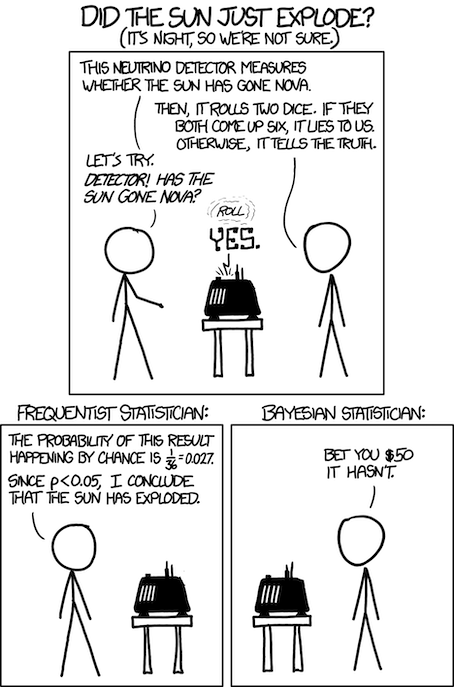
\includegraphics{images/frequentists_vs_bayesians.png}
\end{center}

\setlength{\abovedisplayskip}{-5pt}
\setlength{\abovedisplayshortskip}{-5pt}

{
\hypersetup{linkcolor=}
\setcounter{tocdepth}{2}
\tableofcontents
}
\listoffigures
\listoftables
\hypertarget{prefazione}{%
\chapter*{Prefazione}\label{prefazione}}


\emph{Data Science per psicologi} contiene il materiale delle lezioni dell'insegnamento di \emph{Psicometria B000286} (A.A. 2021/2022) rivolto agli studenti del primo anno del Corso di Laurea in Scienze e Tecniche Psicologiche dell'Università degli Studi di Firenze. \emph{Psicometria} si propone di fornire agli studenti un'introduzione all'analisi dei dati in psicologia. Le conoscenze/competenze che verranno sviluppate in questo insegnamento sono quelle della Data science, ovvero un insieme di conoscenze/competenze che si pongono all'intersezione tra statistica (ovvero, richiedono la capacità di comprendere teoremi statistici) e informatica (ovvero, richiedono la capacità di sapere utilizzare un software).

\hypertarget{la-psicologia-e-la-data-science}{%
\section*{La psicologia e la Data science}\label{la-psicologia-e-la-data-science}}


Sembra sensato spendere due parole su un tema che è importante per gli studenti: quello indicato dal titolo di questo Capitolo. È ovvio che agli studenti di psicologia la statistica non piace. Se piacesse, forse studierebbero Data science e non psicologia; ma non lo fanno. Di conseguenza, gli studenti di psicologia si chiedono: ``perché dobbiamo perdere tanto tempo a studiare queste cose quando in realtà quello che ci interessa è tutt'altro?'' Questa è una bella domanda.

C'è una ragione molto semplice che dovrebbe farci capire perché la Data science è così importante per la psicologia. Infatti, a ben pensarci, la psicologia è una disciplina intrinsecamente statistica, se per statistica intendiamo quella disciplina che studia la variazione delle caratteristiche degli individui nella popolazione. La psicologia studia \emph{gli individui} ed è proprio la variabilità inter- e intra-individuale ciò che vogliamo descrivere e, in certi casi, predire. In questo senso, la psicologia è molto diversa dall'ingegneria, per esempio. Le proprietà di un determinato ponte sotto certe condizioni, ad esempio, sono molto simili a quelle di un altro ponte, sotto le medesime condizioni. Quindi, per un ingegnere la statistica è poco importante: le proprietà dei materiali sono unicamente dipendenti dalla loro composizione e restano costanti. Ma lo stesso non può dirsi degli individui: ogni individuo è unico e cambia nel tempo. E le variazioni tra gli individui, e di un individuo nel tempo, sono l'oggetto di studio proprio della psicologia: è dunque chiaro che i problemi che la psicologia si pone sono molto diversi da quelli affrontati, per esempio, dagli ingegneri. Questa è la ragione per cui abbiamo tanto bisogno della Data science in psicologia: perché la Data science ci consente di descrivere la variazione e il cambiamento. E queste sono appunto le caratteristiche di base dei fenomeni psicologici.

Sono sicuro che, leggendo queste righe, a molti studenti sarà venuta in mente la seguente domanda: perché non chiediamo a qualche esperto di fare il ``lavoro sporco'' (ovvero le analisi statistiche) per noi, mentre noi (gli psicologi) ci occupiamo solo di ciò che ci interessa, ovvero dei problemi psicologici slegati dai dettagli ``tecnici'' della Data science? La risposta a questa domanda è che non è possibile progettare uno studio psicologico sensato senza avere almeno una comprensione rudimentale della Data science. Le tematiche della Data science non possono essere ignorate né dai ricercatori in psicologia né da coloro che svolgono la professione di psicologo al di fuori dell'Università. Infatti, anche i professionisti al di fuori dall'università non possono fare a meno di leggere la letteratura psicologica più recente: il continuo aggiornamento delle conoscenze è infatti richiesto dalla deontologia della professione. Ma per potere fare questo è necessario conoscere un bel po' di Data science! Basta aprire a caso una rivista specialistica di psicologia per rendersi conto di quanto ciò sia vero: gli articoli che riportano i risultati delle ricerche psicologiche sono zeppi di analisi statistiche e di modelli formali. E la comprensione della letteratura psicologica rappresenta un requisito minimo nel bagaglio professionale dello psicologo.

Le considerazioni precedenti cercano di chiarire il seguente punto: la Data science non è qualcosa da studiare a malincuore, in un singolo insegnamento universitario, per poi poterla tranquillamente dimenticare. Nel bene e nel male, gli psicologi usano gli strumenti della Data science in tantissimi ambiti della loro attività professionale: in particolare quando costruiscono, somministrano e interpretano i test psicometrici. È dunque chiaro che possedere delle solide basi di Data science è un tassello imprescindibile del bagaglio professionale dello psicologo. In questo insegnamento verrano trattati i temi base della Data science e verrà adottato un punto di vista bayesiano, che corrisponde all'approccio più recente e sempre più diffuso in psicologia.

\hypertarget{come-studiare}{%
\section*{Come studiare}\label{come-studiare}}


Il giusto metodo di studio per prepararsi all'esame di Psicometria è quello di seguire attivamente le lezioni, assimilare i concetti via via che essi vengono presentati e verificare in autonomia le procedure presentate a lezione. Incoraggio gli studenti a farmi domande per chiarire ciò che non è stato capito appieno. Incoraggio gli studenti a utilizzare i forum attivi su Moodle e, soprattutto, a svolgere gli esercizi proposti su Moodle. I problemi forniti su Moodle rappresentano il livello di difficoltà richiesto per superare l'esame e consentono allo studente di comprendere se le competenze sviluppate fino a quel punto sono sufficienti rispetto alle richieste dell'esame.

La prima fase dello studio, che è sicuramente individuale, è quella in cui è necessario acquisire le conoscenze teoriche relative ai problemi che saranno presentati all'esame. La seconda fase di studio, che può essere facilitata da scambi con altri e da incontri di gruppo, porta ad acquisire la capacità di applicare le conoscenze: è necessario capire come usare un software (\(\textsf{R}\)) per applicare i concetti statistici alla specifica situazione del problema che si vuole risolvere. Le due fasi non sono però separate: il saper fare molto spesso ci aiuta a capire meglio.

\hypertarget{sviluppare-un-metodo-di-studio-efficace}{%
\section*{Sviluppare un metodo di studio efficace}\label{sviluppare-un-metodo-di-studio-efficace}}


Avendo insegnato molte volte in passato un corso introduttivo di analisi dei dati ho notato nel corso degli anni che gli studenti con l'atteggiamento mentale che descriverò qui sotto generalmente ottengono ottimi risultati. Alcuni studenti sviluppano naturalmente questo approccio allo studio, ma altri hanno bisogno di fare uno sforzo per maturarlo. Fornisco qui sotto una breve descrizione del ``metodo di studio'' che, nella mia esperienza, è il più efficace per affrontare le richieste di questo insegnamento.

\begin{itemize}
\tightlist
\item
  Dedicate un tempo sufficiente al materiale di base, apparentemente facile; assicuratevi di averlo capito bene. Cercate le lacune nella vostra comprensione. Leggere presentazioni diverse dello stesso materiale (in libri o articoli diversi) può fornire nuove intuizioni.
\item
  Gli errori che facciamo sono i nostri migliori maestri. Istintivamente cerchiamo di dimenticare subito i nostri errori. Ma il miglior modo di imparare è apprendere dagli errori che commettiamo. In questo senso, una soluzione corretta è meno utile di una soluzione sbagliata. Quando commettiamo un errore questo ci fornisce un'informazione importante: ci fa capire qual è il materiale di studio sul quale dobbiamo ritornare e che dobbiamo capire meglio.
\item
  C'è ovviamente un aspetto ``psicologico'' nello studio. Quando un esercizio o problema ci sembra incomprensibile, la cosa migliore da fare è dire: ``mi arrendo'', ``non ho idea di cosa fare!''. Questo ci rilassa: ci siamo già arresi, quindi non abbiamo niente da perdere, non dobbiamo più preoccuparci. Ma non dobbiamo fermarci qui. Le cose ``migliori'' che faccio (se ci sono) le faccio quando non ho voglia di lavorare. Alle volte, quando c'è qualcosa che non so fare e non ho idea di come affontare, mi dico: ``oggi non ho proprio voglia di fare fatica'', non ho voglia di mettermi nello stato mentale per cui ``in 10 minuti devo risolvere il problema perché dopo devo fare altre cose''. Però ho voglia di \emph{divertirmi} con quel problema e allora mi dedico a qualche aspetto ``marginale'' del problema, che so come affrontare, oppure considero l'aspetto più difficile del problema, quello che non so come risolvere, ma invece di cercare di risolverlo, guardo come altre persone hanno affrontato problemi simili, opppure lo stesso problema in un altro contesto. Non mi pongo l'obiettivo ``risolvi il problema in 10 minuti'', ma invece quello di farmi un'idea ``generale'' del problema, o quello di capire un caso più specifico e più semplice del problema. Senza nessuna pressione. Infatti, in quel momento ho deciso di non lavorare (ovvero, di non fare fatica). Va benissimo se ``parto per la tangente'', ovvero se mi metto a leggere del materiale che sembra avere poco a che fare con il problema centrale (le nostre intuizioni e la nostra curiosità solitamente ci indirizzano sulla strada giusta). Quando faccio così, molto spesso trovo la soluzione del problema che mi ero posto e, paradossalmente, la trovo in un tempo minore di quello che, in precedenza, avevo dedicato a ``lavorare'' al problema. Allora perché non faccio sempre così? C'è ovviamente l'aspetto dei ``10 minuti'' che non è sempre facile da dimenticare. Sotto pressione, possiamo solo agire in maniera automatica, ovvero possiamo solo applicare qualcosa che già sappiamo fare. Ma se dobbiamo imparare qualcosa di nuovo, la pressione è un impedimento.
\item
  È utile farsi da soli delle domande sugli argomenti trattati, senza limitarsi a cercare di risolvere gli esercizi che vengono assegnati. Quando studio qualcosa mi viene in mente: ``se questo è vero, allora deve succedere quest'altra cosa''. Allora verifico se questo è vero, di solito con una simulazione. Se i risultati della simulazione sono quelli che mi aspetto, allora vuol dire che ho capito. Se i risultati sono diversi da quelli che mi aspettavo, allora mi rendo conto di non avere capito e ritorno indietro a studiare con più attenzione la teoria che pensavo di avere capito -- e ovviamente mi rendo conto che c'era un aspetto che avevo frainteso. Questo tipo di verifica è qualcosa che dobbiamo fare da soli, in prima persona: nessun altro può fare questo al posto nostro.
\item
  Non aspettatevi di capire tutto la prima volta che incontrate un argomento nuovo.\footnote{Ricordatevi inoltre che gli individui tendono a sottostimare la propria capacità di apprendere \citep{horn2021underestimating}.} È utile farsi una nota mentalmente delle lacune nella vostra comprensione e tornare su di esse in seguito per carcare di colmarle. L'atteggiamento naturale, quando non capiamo i dettagli di qualcosa, è quello di pensare: ``non importa, ho capito in maniera approssimativa questo punto, non devo preoccuparmi del resto''. Ma in realtà non è vero: se la nostra comprensione è superficiale, quando il problema verrà presentato in una nuova forma, non riusciremo a risolverlo. Per cui i dubbi che ci vengono quando studiamo qualcosa sono il nostro alleato più prezioso: ci dicono esattamente quali sono gli aspetti che dobbiamo approfondire per potere migliorare la nostra preparazione.
\item
  È utile sviluppare una visione d'insieme degli argomenti trattati, capire l'obiettivo generale che si vuole raggiungere e avere chiaro il contributo che i vari pezzi di informazione forniscono al raggiungimento di tale obiettivo. Questa organizzazione mentale del materiale di studio facilita la comprensione. È estremamente utile creare degli schemi di ciò che si sta studiando. Non aspettate che sia io a fornirvi un riepilogo di ciò che dovete imparare: sviluppate da soli tali schemi e tali riassunti.
\item
  Tutti noi dobbiamo imparare l'arte di trovare le informazioni, non solo nel caso di questo insegnamento. Quando vi trovate di fronte a qualcosa che non capite, o ottenete un oscuro messaggio di errore da un software, ricordatevi: ``Google is your friend''!
\end{itemize}

\begin{flushright}
Corrado Caudek\\
Marzo 2022 \end{flushright}

\mainmatter

\hypertarget{part-il-calcolo-delle-probabilituxe0}{%
\part{Il calcolo delle probabilità}\label{part-il-calcolo-delle-probabilituxe0}}

\hypertarget{intro-prob-1}{%
\chapter{La logica dell'incerto}\label{intro-prob-1}}

In questa parte della dispensa verrà introdotta la teoria delle probabilità. Prima di entrare nei dettagli, cerchiamo di capire perché la probabilità sia cruciale per la ricerca scientifica.

La teoria delle probabilità è cruciale per la scienza perché la ricerca procede mediante l'inferenza induttiva. Non siamo mai completamente sicuri della verità di una proposizione (ipotesi, teoria): al valore di verità di una proposizione possiamo solo assegnare un giudizio probabilistico. L'approccio bayesiano è una scuola di pensiero che usa la probabilità per quantificare il grado di fiducia che può essere attribuito ad una proposizione. L'inferenza statistica bayesiana è un tipo di inferenza induttiva che ha lo scopo di quantificare la fiducia che si ha nell'ipotesi \(H\) dopo il verificarsi del dato d'evidenza \(E\). Per quantificare un tale grado di fiducia l'inferenza statistica bayesiana utilizza la teoria delle probabilità. Una comprensione dell'inferenza statistica bayesiana richiede dunque, preliminarmente, la conoscenze della teoria delle probabilità.

\hypertarget{che-cosuxe8-la-probabilituxe0}{%
\section{Che cos'è la probabilità?}\label{che-cosuxe8-la-probabilituxe0}}

La definizione della probabilità è un problema estremamente dibattuto ed aperto. Sono state fornite due possibili soluzioni al problema di definire il concetto di probabilità.

\begin{enumerate}
\def\labelenumi{(\alph{enumi})}
\item
  La natura della probabilità è ``ontologica'' (ovvero, basata sulla metafisica): la probabilità è una proprietà della della realtà, del mondo, di come sono le cose, indipendentemente dalla nostra esperienza. È una visione che qualcuno chiama ``oggettiva''.
\item
  La natura della probabilità è ``epistemica'' (ovvero, basata sulla conoscenza): la probabilità si riferisce alla conoscenza che abbiamo del mondo, non al mondo in sé. Di conseguenza è detta, in contrapposizione alla precedente definizione, ``soggettiva''.
\end{enumerate}

In termini epistemici, la probabilità fornisce una misura della nostra incertezza sul verificarsi di un fenomeno, alla luce delle informazioni disponibili. Potremmo dire che c'è una ``scala'' naturale che ha per estremi il vero (1: evento certo) da una parte ed il falso (0: evento impossibile) dall'altra. La probabilità è la quantificazione di questa scala: descrive lo stato della nostra incertezza rispetto al contenuto di verità di una proposizione.

L'incertezza nelle nostre previsioni può sorgere per due ragioni fondamentalmente diverse. Il primo è dovuto alla nostra ignoranza delle cause nascoste sottostanti o dei meccanismi che generano i dati. Questa è appunto un'incertezza \emph{epistemica}. Il secondo tipo di incertezza deriva dalla variabilità intrinseca dei fenomeni, che non può essere ridotta anche se raccogliamo più dati. Questa seconda forma di incertezza è talvolta chiamata \emph{aleatoria}. Come esempio concreto, consideriamo il lancio di una moneta equilibrata. Sappiamo con certezza che la probabilità di testa è \(P = 0.5\), quindi non c'è incertezza epistemica, ma non questo non è sufficiente per prevedere con certezza il risultato -- ovvero, l'incertezza aleatoria persiste anche in assenza di incertezza epistemica.

Nell'interpretazione frequentista, la probabilità \(P(E)\) rappresenta la frequenza relativa a lungo termine di un grande numero di ripetizioni di un esperimento casuale sotto le medesime condizioni. Viene stressata qui l'idea che ciò di cui parliamo è qualcosa che emerge nel momento in cui è possibile ripetere l'esperimento casuale tante volte sotto le medesime condizioni -- sono invece esclusi gli eventi unici e irripetibili.

L'interpretazione bayesiana della probabilità fa invece ricorso ad una concezione più ampia, non legata al solo evento in sé ma che include anche il soggetto assegnante la funzione di probabilità. In pratica l'assegnazione di probabilità bayesiana viene effettuata dal decisore, in base alle proprie conoscenze a priori integrate con tutto il generico bagaglio culturale personale. In questo modo, la probabilità non sarà obbligatoriamente la stessa per tutti i soggetti, ma variarierà a seconda delle informazioni a disposizione, dell'esperienza personale e soprattutto del punto di vista proprio di ogni decisore ed è dunque assimilabile al ``grado di fiducia'' -- in inglese \emph{degree of belief} -- di un dato soggetto, in un dato istante e con un dato insieme d'informazioni, circa l'accadere dell'evento \(E\). ``{[}N{]}essuna scienza ci permetterà di dire: il tale fatto accadrà, andrà così e così, perché ciò è conseguenza di tale legge, e tale legge è una verità assoluta, ma tanto meno ci condurrà a concludere scetticamente: la verità assoluta non esiste, e quindi tale fatto può accadere e può non accadere, può andare così e può andare in tutt'altro modo, nulla io ne so. Quel che si potrà dire è questo: io prevedo che il tale fatto avverrà, e avverrà nel tal modo, perché l'esperienza del passato e l'elaborazione scientifica cui il pensiero dell'uomo l'ha sottoposta mi fanno sembrare ragionevole questa previsione'' \citep{definetti1931prob}.

L'impostazione bayesiana, sviluppata da Ramsey e de Finetti, riconduce l'assegnazione di probabilità allo scommettere sul verificarsi di un evento: la probabilità di un evento \(E\) è la quota \(p(E)\) che un individuo reputa di dover pagare ad un banco per ricevere ``1'' ovvero ``0'' verificandosi o non verificandosi \(E\).

Secondo De Finetti, le valutazioni di probabilità degli eventi devono rispondere ai principi di equità e coerenza. Una scommessa risponde al principio di \emph{equità} se il ruolo di banco e giocatore sono scambiabili in ogni momento del gioco e sempre alle stesse condizioni. Una scommessa risponde al principio di \emph{coerenza} se non vi sono combinazioni di scommesse che consentano (sia al banco che al giocatore) di realizzare perdite o vincite certe.

L'approccio definettiano dell'impostazione della scommessa si basa dunque sulle assunzioni di razionalità e coerenza del decisore, al quale è fatto esplicito divieto di effettuare scommesse a perdita o guadagno certo. Il decisore, proponendo la scommessa, deve essere disposto a scambiare il posto dello scommettitore con quello del banco.

Il metodo della scommessa, oltre che una definizione, fornisce un mezzo operativo di assegnazione della probabilità. Sulla base di questa definizione operativa, che si può ritenere ragionevolmente soddisfatta dal comportamento di un qualunque individuo che agisca in modo razionale in condizioni di incertezza, possono essere agevolmente dimostrate tutte le proprietà classiche della probabilità: essa non può assumere valori negativi, né può essere superiore all'unità; se \(E\) è un evento certo, la sua probabilità è 1; se invece \(E\) è un evento impossibile, la sua probabilità è 0.

I problemi posti dall'approccio definettiano riguardano l'arbitrarietà dell'assegnazione soggettività di probabilità la quale sembra negare la validità dell'intero costrutto teorico. In risposta a tale critica, i bayesiani sostengono che gli approcci oggettivisti alla probabilità nascondono scelte arbitrarie preliminari e sono basate su assunzioni implausibili. È molto più onesto esplicitare subito tutte le scelte arbitrarie effettuate nel corso dell'analisi in modo da controllarne coerenza e razionalità.

\hypertarget{variabili-casuali-e-probabilituxe0-di-un-evento}{%
\section{Variabili casuali e probabilità di un evento}\label{variabili-casuali-e-probabilituxe0-di-un-evento}}

Esaminiamo qui di seguito alcuni concetti di base della teoria delle probabilità, la quale può essere vista come un'estensione della logica.

\hypertarget{eventi-e-probabilituxe0}{%
\subsection{Eventi e probabilità}\label{eventi-e-probabilituxe0}}

Nella teoria delle probabilità il risultato ``testa'' nel lancio di una moneta è chiamato \emph{evento}.\footnote{Per un ripasso delle nozioni di base della teoria degli insiemi, si veda l'Appendice \ref{insiemistica}.} Un evento, denotato da una variabile binaria, corrisponde ad uno stato del mondo che si verifica oppure no. Ad esempio, \(Y\) = 1 può denotare l'evento per cui il lancio di una moneta produce il risultato testa. Il funzionale \(P(Y)\) denota la probabilità con cui si ritiene che l'evento \(Y\) sia vero (o la proporzione di volte che si verifica tale evento osservando a lungo termine delle ripetizioni indipendenti di un esperimento casuale). Ad esempio, per il lancio di una moneta equilibrata, la probabilità dell'evento ``il risultato del lancio della moneta è testa'' è scritta come \(P(Y = 1) = 0.5.\)

Se la moneta è equilibrata dobbiamo anche avere \(P(Y = 0) = 0.5\). I due eventi \emph{Y} = 1 e \(Y\) = 0 sono \emph{mutuamente esclusivi} nel senso che non possono entrambi verificarsi contemporaneamente: \(P(Y = 1\; \land \; Y = 0) = 0.\) Gli eventi \(Y\) = 1 e \(Y\) = 0 di dicono \emph{esaustivi}, nel senso che almeno uno di essi deve verificarsi e nessun altro tipo di evento è possibile. Nella notazione probabilistica, \(P(Y = 1\; \lor \; Y = 0) = 1.\) Il connettivo logico ``o'' (\(\lor\)) specifica eventi \emph{disgiunti}, ovvero eventi che non possono verificarsi contemporaneamente (eventi \emph{incompatibili}) e per i quali, perciò, la probabilità della loro congiunzione è \(P(A \; \land \; B) = 0\). Il connettivo logico ``e'' (\(\land\)), invece, specifica eventi \emph{congiunti}, ovvero eventi che possono verificarsi contemporaneamente (eventi \emph{compatibili}) e per i quali, perciò, la probabilità della loro congiunzione è \(P(A \; \land \; B) > 0\). La probabilità del verificarsi di due eventi congiunti \(A\) e \(B\) si può denotare, in maniera equivalente, con la notazione precedente, oppure con \(P(A \cap B)\), oppure con \(P(A, B)\).

Si richiede che \(0 \leq P(A) \leq 1\), dove \(P(A) = 0\) denota l'evento impossibile e \(P(A) = 1\) denota l'evento certo. Scriviamo \(P(\lnot A)\) o \(P(\bar{A})\) per denotare la probabilità che l'evento \(A\) non avvenga; questa probabilità è definita come \(P(\bar{A}) = 1 − P(A)\).

\hypertarget{spazio-campione-e-risultati-possibili}{%
\subsection{Spazio campione e risultati possibili}\label{spazio-campione-e-risultati-possibili}}

Anche se il lancio di una moneta produce sempre uno specifico risultato nel mondo reale, possiamo anche immaginare i possibili risultati alternativi che si sarebbero potuti osservare. Quindi, anche se in uno specifico lancio la moneta dà testa (\(Y\) = 1), possiamo immaginare la possibilità che il lancio possa avere prodotto croce (\(Y\) = 0). Tale ragionamento controfattuale è la chiave per comprendere la teoria delle probabilità e l'inferenza statistica.

I risultati possibili che si possono osservare come conseguenza del lancio di una moneta determinano i valori possibili che la variabile casuale può assumere. L'insieme \(\Omega\) di tutti i risultati possibili è chiamato \emph{spazio campione} (\emph{sample space}). Lo spazio campione può essere concettualizzato come un'urna contenente una pallina per ogni possibile risultato del lancio della moneta. Su ogni pallina è scritto il valore della variabile casuale. Uno specifico lancio di una moneta -- ovvero, l'osservazione di uno specifico valore di una variabile casuale -- è chiamato \emph{esperimento casuale}.

Il lancio di un dado ci fornisce l'esempio di un altro esperimento casuale. Supponiamo di essere interessati all'evento ``il lancio del dado produce un numero dispari''. Un \emph{evento} seleziona un sottoinsieme dello spazio campione: in questo caso, l'insieme dei risultati \(\{1, 3, 5\}\). Se esce 3, per esempio, diciamo che si è verificato l'evento ``dispari'' (ma l'evento ``dispari'' si sarebbe anche verificato anche se fosse uscito 1 o 5).

\hypertarget{variabili-casuali}{%
\section{Variabili casuali}\label{variabili-casuali}}

Sia \(Y\) il risultato del lancio di moneta equilibrata, non di un generico lancio di una moneta, ma un'istanza specifica del lancio di una specifica moneta in un dato momento. Definita in questo modo, \(Y\) è una \emph{variabile casuale}, ovvero una variabile i cui valori non possono essere previsti con esattezza. Se la moneta è equilibrata, c'è una probabilità del 50\% che il lancio della moneta dia come risultato ``testa'' e una probabilità del 50\% che dia come risultato ``croce''. Per facilitare la trattazione, le variabili casuali assumono solo valori numerici. Per lo specifico lancio della moneta in questione, diciamo, ad esempio, che la variabile casuale \(Y\) assume il valore 1 se esce testa e il valore 0 se esce croce.

Una variabile casuale può essere \emph{discreta} o \emph{continua}. Una variabile casuale discreta può assumere un numero finito di valori \(x_1, \dots ,x_n\), in corrispondenza degli eventi \(E_i, \dots, E_n\) che si verificano con le rispettive probabilità \(p_1, \dots, p_n\). Un esempio è il punteggio totale di un test psicometrico costituito da item su scala Likert. Invece un esempio di una variabile casuale continua è la distanza tra due punti, che può assumere infiniti valori all'interno di un certo intervallo. L'insieme \(S\) dei valori che la variabile casuale può assumere è detto \emph{spazio dei valori} o \emph{spazio degli stati}. La caratteristica fondamentale di una variabile casuale è data dall'insieme delle probabilità dei suoi valori, detta \emph{distribuzione di probabilità}. Nel seguito useremo la notazione \(P(\cdot)\) per fare riferimento alle distribuzioni di probabilità delle variabili casuali discrete e \(p(\cdot)\) per fare riferimento alla densità di probabilità delle variabili casuali continue. In questo contesto, l'insieme dei valori che la variabile casuale può assumere è detto \emph{supporto} della sua distribuzione di probabilità. Il supporto di una variabile casuale può essere finito (come nel caso di una variabile casuale uniforme di supporto \([a, b]\)) o infinito (nel caso di una variabile causale gaussiana il cui supporto coincide con la retta reale).

\hypertarget{usare-la-simulazione-per-stimare-le-probabilituxe0}{%
\section{Usare la simulazione per stimare le probabilità}\label{usare-la-simulazione-per-stimare-le-probabilituxe0}}

In questa dispensa verrà adottata l'interpretazione bayesiana delle probabilità. Tuttavia, le regole di base della teoria delle probabilità sono le stesse, indipendentemente dall'interpretazione adottata. Pertanto, negli esempi seguenti, possiamo utilizzare la simulazione per stimarere le probabilità degli eventi in un modo diretto, ovvero mediante la generazione di molteplici osservazioni delle variabili casuali derivate dagli eventi di interesse. Ad esempio, per simulare in \(\R\) il lancio di una moneta equilibrata iniziamo con il definire un vettore che contiene i risultati possibili del lancio della moneta (ovvero i valori possibili della variabile casuale \(Y\)):

\begin{Shaded}
\begin{Highlighting}[]
\NormalTok{coin }\OtherTok{\textless{}{-}} \FunctionTok{c}\NormalTok{(}\DecValTok{0}\NormalTok{, }\DecValTok{1}\NormalTok{)}
\end{Highlighting}
\end{Shaded}

L'estrazione casuale di uno di questi due possibili valori (ovvero, la simulazione di uno specifico lancio di una moneta) si realizza con la funzione \texttt{sample()}:

\begin{Shaded}
\begin{Highlighting}[]
\FunctionTok{sample}\NormalTok{(coin, }\AttributeTok{size =} \DecValTok{1}\NormalTok{)}
\CommentTok{\#\textgreater{} [1] 0}
\end{Highlighting}
\end{Shaded}

In maniera equivalente, la stessa operazione si può realizzare mediante l'istruzione

\begin{Shaded}
\begin{Highlighting}[]
\FunctionTok{rbinom}\NormalTok{(}\DecValTok{1}\NormalTok{, }\DecValTok{1}\NormalTok{, }\FloatTok{0.5}\NormalTok{)}
\CommentTok{\#\textgreater{} [1] 1}
\end{Highlighting}
\end{Shaded}

Supponiamo di ripetere questo esperimento casuale 100 volte e di registrare i risultati così ottenuti. La stima della probabilità dell'evento \(P(Y = 1)\) è data dalla frequenza relativa del numero di volte in cui abbiamo osservato l'evento di interesse (\(Y = 1\)):

\begin{Shaded}
\begin{Highlighting}[]
\NormalTok{M }\OtherTok{\textless{}{-}} \DecValTok{100}
\NormalTok{y }\OtherTok{\textless{}{-}} \FunctionTok{rep}\NormalTok{(}\ConstantTok{NA}\NormalTok{, M)}
\ControlFlowTok{for}\NormalTok{ (m }\ControlFlowTok{in} \DecValTok{1}\SpecialCharTok{:}\NormalTok{M) \{}
\NormalTok{  y[m] }\OtherTok{\textless{}{-}} \FunctionTok{rbinom}\NormalTok{(}\DecValTok{1}\NormalTok{, }\DecValTok{1}\NormalTok{, }\FloatTok{0.5}\NormalTok{)}
\NormalTok{\}}
\NormalTok{estimate }\OtherTok{\textless{}{-}} \FunctionTok{sum}\NormalTok{(y) }\SpecialCharTok{/}\NormalTok{ M}

\FunctionTok{cat}\NormalTok{(}\StringTok{"estimated Pr[Y = 1] ="}\NormalTok{, estimate)}
\CommentTok{\#\textgreater{} estimated Pr[Y = 1] = 0.53}
\end{Highlighting}
\end{Shaded}

Ripetiamo questa procedura 10 volte.

\begin{Shaded}
\begin{Highlighting}[]
\NormalTok{flip\_coin }\OtherTok{\textless{}{-}} \ControlFlowTok{function}\NormalTok{(M) \{}
\NormalTok{  y }\OtherTok{\textless{}{-}} \FunctionTok{rep}\NormalTok{(}\ConstantTok{NA}\NormalTok{, M)}
  \ControlFlowTok{for}\NormalTok{ (m }\ControlFlowTok{in} \DecValTok{1}\SpecialCharTok{:}\NormalTok{M) \{}
\NormalTok{    y[m] }\OtherTok{\textless{}{-}} \FunctionTok{rbinom}\NormalTok{(}\DecValTok{1}\NormalTok{, }\DecValTok{1}\NormalTok{, }\FloatTok{0.5}\NormalTok{)}
\NormalTok{  \}}
\NormalTok{  estimate }\OtherTok{\textless{}{-}} \FunctionTok{sum}\NormalTok{(y) }\SpecialCharTok{/}\NormalTok{ M}
  \FunctionTok{cat}\NormalTok{(}\StringTok{"estimated Pr[Y = 1] ="}\NormalTok{, estimate, }\StringTok{"}\SpecialCharTok{\textbackslash{}n}\StringTok{"}\NormalTok{)}
\NormalTok{\}}
\end{Highlighting}
\end{Shaded}

\begin{Shaded}
\begin{Highlighting}[]
\ControlFlowTok{for}\NormalTok{ (i }\ControlFlowTok{in} \DecValTok{1}\SpecialCharTok{:}\DecValTok{10}\NormalTok{) \{}
  \FunctionTok{flip\_coin}\NormalTok{(}\DecValTok{100}\NormalTok{)}
\NormalTok{\}}
\CommentTok{\#\textgreater{} estimated Pr[Y = 1] = 0.44 }
\CommentTok{\#\textgreater{} estimated Pr[Y = 1] = 0.52 }
\CommentTok{\#\textgreater{} estimated Pr[Y = 1] = 0.46 }
\CommentTok{\#\textgreater{} estimated Pr[Y = 1] = 0.57 }
\CommentTok{\#\textgreater{} estimated Pr[Y = 1] = 0.47 }
\CommentTok{\#\textgreater{} estimated Pr[Y = 1] = 0.46 }
\CommentTok{\#\textgreater{} estimated Pr[Y = 1] = 0.48 }
\CommentTok{\#\textgreater{} estimated Pr[Y = 1] = 0.49 }
\CommentTok{\#\textgreater{} estimated Pr[Y = 1] = 0.47 }
\CommentTok{\#\textgreater{} estimated Pr[Y = 1] = 0.62}
\end{Highlighting}
\end{Shaded}

Dato che la moneta è equilibrata, la stima delle probabilità dell'evento \(Pr[Y = 1]\) è simile a al valore che ci aspettiamo, ovvero \(P(Y = 1)\) = 0.5, ma il risultato ottenuto nelle simulazioni non è sempre esatto. Proviamo ad aumentare il numero di lanci in ciascuna simulazione:

\begin{Shaded}
\begin{Highlighting}[]
\ControlFlowTok{for}\NormalTok{ (i }\ControlFlowTok{in} \DecValTok{1}\SpecialCharTok{:}\DecValTok{10}\NormalTok{) \{}
  \FunctionTok{flip\_coin}\NormalTok{(}\DecValTok{1000}\NormalTok{)}
\NormalTok{\}}
\CommentTok{\#\textgreater{} estimated Pr[Y = 1] = 0.497 }
\CommentTok{\#\textgreater{} estimated Pr[Y = 1] = 0.529 }
\CommentTok{\#\textgreater{} estimated Pr[Y = 1] = 0.493 }
\CommentTok{\#\textgreater{} estimated Pr[Y = 1] = 0.511 }
\CommentTok{\#\textgreater{} estimated Pr[Y = 1] = 0.506 }
\CommentTok{\#\textgreater{} estimated Pr[Y = 1] = 0.52 }
\CommentTok{\#\textgreater{} estimated Pr[Y = 1] = 0.49 }
\CommentTok{\#\textgreater{} estimated Pr[Y = 1] = 0.495 }
\CommentTok{\#\textgreater{} estimated Pr[Y = 1] = 0.489 }
\CommentTok{\#\textgreater{} estimated Pr[Y = 1] = 0.496}
\end{Highlighting}
\end{Shaded}

In questo secondo caso, gli errori tendono ad essere più piccoli che nel caso precedente. Cosa succede se in ciascuna simulazione esaminiamo i risultati di 10,000 lanci della moneta?

\begin{Shaded}
\begin{Highlighting}[]
\ControlFlowTok{for}\NormalTok{ (i }\ControlFlowTok{in} \DecValTok{1}\SpecialCharTok{:}\DecValTok{10}\NormalTok{) \{}
  \FunctionTok{flip\_coin}\NormalTok{(}\FloatTok{1e4}\NormalTok{)}
\NormalTok{\}}
\CommentTok{\#\textgreater{} estimated Pr[Y = 1] = 0.4885 }
\CommentTok{\#\textgreater{} estimated Pr[Y = 1] = 0.4957 }
\CommentTok{\#\textgreater{} estimated Pr[Y = 1] = 0.4902 }
\CommentTok{\#\textgreater{} estimated Pr[Y = 1] = 0.5032 }
\CommentTok{\#\textgreater{} estimated Pr[Y = 1] = 0.5048 }
\CommentTok{\#\textgreater{} estimated Pr[Y = 1] = 0.4931 }
\CommentTok{\#\textgreater{} estimated Pr[Y = 1] = 0.4965 }
\CommentTok{\#\textgreater{} estimated Pr[Y = 1] = 0.499 }
\CommentTok{\#\textgreater{} estimated Pr[Y = 1] = 0.4979 }
\CommentTok{\#\textgreater{} estimated Pr[Y = 1] = 0.4973}
\end{Highlighting}
\end{Shaded}

Ora le stime ottenute sono molto vicine alla vera probabilità che vogliamo stimare (cioè 0.5, perché la moneta è equilibrata). I risultati delle simulazioni precedenti pongono dunque il problema di determinare quale sia il numero di lanci di cui abbiamo bisogno per assicurarci che le stime siano accurate (ovvero, vicine al valore corretto della probabilità)

\hypertarget{la-legge-dei-grandi-numeri}{%
\section{La legge dei grandi numeri}\label{la-legge-dei-grandi-numeri}}

La visualizzazione mediante grafici contribuisce alla comprensione dei concetti della statistica e della teoria delle probabilità. Un modo per descrivere ciò che accade all'aumentare del numero \(M\) di ripetizioni del lancio della moneta consiste nel registrare la stima della probabilità dell'evento \(P(Y = 1)\) in funzione del numero di ripetizioni dell'esperimento casuale per ogni \(m \in 1:M\). Possiamo ottenere un grafico dell'andamento della stima di \(P(Y = 1)\) in funzione di \(m\) nel modo seguente:

\begin{Shaded}
\begin{Highlighting}[]
\NormalTok{nrep }\OtherTok{\textless{}{-}} \FloatTok{1e4}
\NormalTok{estimate }\OtherTok{\textless{}{-}} \FunctionTok{rep}\NormalTok{(}\ConstantTok{NA}\NormalTok{, nrep)}
\NormalTok{flip\_coin }\OtherTok{\textless{}{-}} \ControlFlowTok{function}\NormalTok{(m) \{}
\NormalTok{  y }\OtherTok{\textless{}{-}} \FunctionTok{rbinom}\NormalTok{(m, }\DecValTok{1}\NormalTok{, }\FloatTok{0.5}\NormalTok{)}
\NormalTok{  phat }\OtherTok{\textless{}{-}} \FunctionTok{sum}\NormalTok{(y) }\SpecialCharTok{/}\NormalTok{ m}
\NormalTok{  phat}
\NormalTok{\}}
\ControlFlowTok{for}\NormalTok{ (i }\ControlFlowTok{in} \DecValTok{1}\SpecialCharTok{:}\NormalTok{nrep) \{}
\NormalTok{  estimate[i] }\OtherTok{\textless{}{-}} \FunctionTok{flip\_coin}\NormalTok{(i)}
\NormalTok{\}}
\NormalTok{d }\OtherTok{\textless{}{-}} \FunctionTok{tibble}\NormalTok{(}
  \AttributeTok{n =} \DecValTok{1}\SpecialCharTok{:}\NormalTok{nrep,}
\NormalTok{  estimate}
\NormalTok{)}
\NormalTok{d }\SpecialCharTok{\%\textgreater{}\%}
  \FunctionTok{ggplot}\NormalTok{(}\FunctionTok{aes}\NormalTok{(}\AttributeTok{x =}\NormalTok{ n, }\AttributeTok{y =}\NormalTok{ estimate)) }\SpecialCharTok{+}
  \FunctionTok{geom\_line}\NormalTok{() }\SpecialCharTok{+}
  \FunctionTok{labs}\NormalTok{(}
    \AttributeTok{x =} \StringTok{"Numero di lanci della moneta"}\NormalTok{,}
    \AttributeTok{y =} \StringTok{"Stima di P(Y = 1)"}
\NormalTok{  )}
\end{Highlighting}
\end{Shaded}

\begin{figure}

{\centering 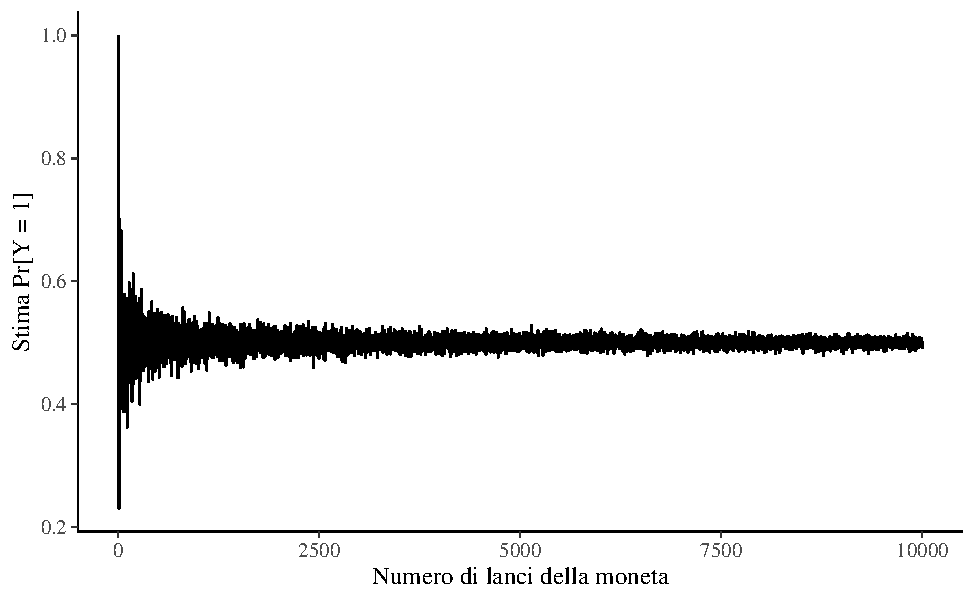
\includegraphics{ds4psy_files/figure-latex/legge-grandi-n-1-1} 

}

\caption{Stima della probabilità di successo in funzione del numero dei lanci di una moneta.}\label{fig:legge-grandi-n-1}
\end{figure}

Dato che la figura \ref{fig:legge-grandi-n-1} espressa su una scala lineare non rivela chiaramente l'andamento della simulazione, imponiamo una scala logaritmica sull'asse delle ascisse (\(x\)). Su scala logaritmica, i valori tra 1 e 10 vengono tracciati all'incirca con la stessa ampiezza che si osserva tra i valori 50 e 700, eccetera.

\begin{Shaded}
\begin{Highlighting}[]
\NormalTok{d }\SpecialCharTok{\%\textgreater{}\%}
  \FunctionTok{ggplot}\NormalTok{(}\FunctionTok{aes}\NormalTok{(}\AttributeTok{x =}\NormalTok{ n, }\AttributeTok{y =}\NormalTok{ estimate)) }\SpecialCharTok{+}
  \FunctionTok{geom\_line}\NormalTok{() }\SpecialCharTok{+}
  \FunctionTok{geom\_hline}\NormalTok{(}
    \AttributeTok{yintercept =} \FloatTok{0.5}\NormalTok{, }\AttributeTok{color =} \StringTok{"gray"}\NormalTok{, }\AttributeTok{size =} \DecValTok{1}
\NormalTok{  ) }\SpecialCharTok{+}
  \FunctionTok{scale\_x\_log10}\NormalTok{(}
    \AttributeTok{breaks =} \FunctionTok{c}\NormalTok{(}
      \DecValTok{1}\NormalTok{, }\DecValTok{3}\NormalTok{, }\DecValTok{10}\NormalTok{, }\DecValTok{50}\NormalTok{, }\DecValTok{200}\NormalTok{,}
      \DecValTok{700}\NormalTok{, }\DecValTok{2500}\NormalTok{, }\DecValTok{10000}
\NormalTok{    )}
\NormalTok{  ) }\SpecialCharTok{+}
  \FunctionTok{labs}\NormalTok{(}
    \AttributeTok{x =} \StringTok{"Numero dei lanci della moneta (scala logaritmica)"}\NormalTok{,}
    \AttributeTok{y =} \StringTok{"Stima di P(Y = 1)"}
\NormalTok{  )}
\end{Highlighting}
\end{Shaded}

\begin{figure}

{\centering 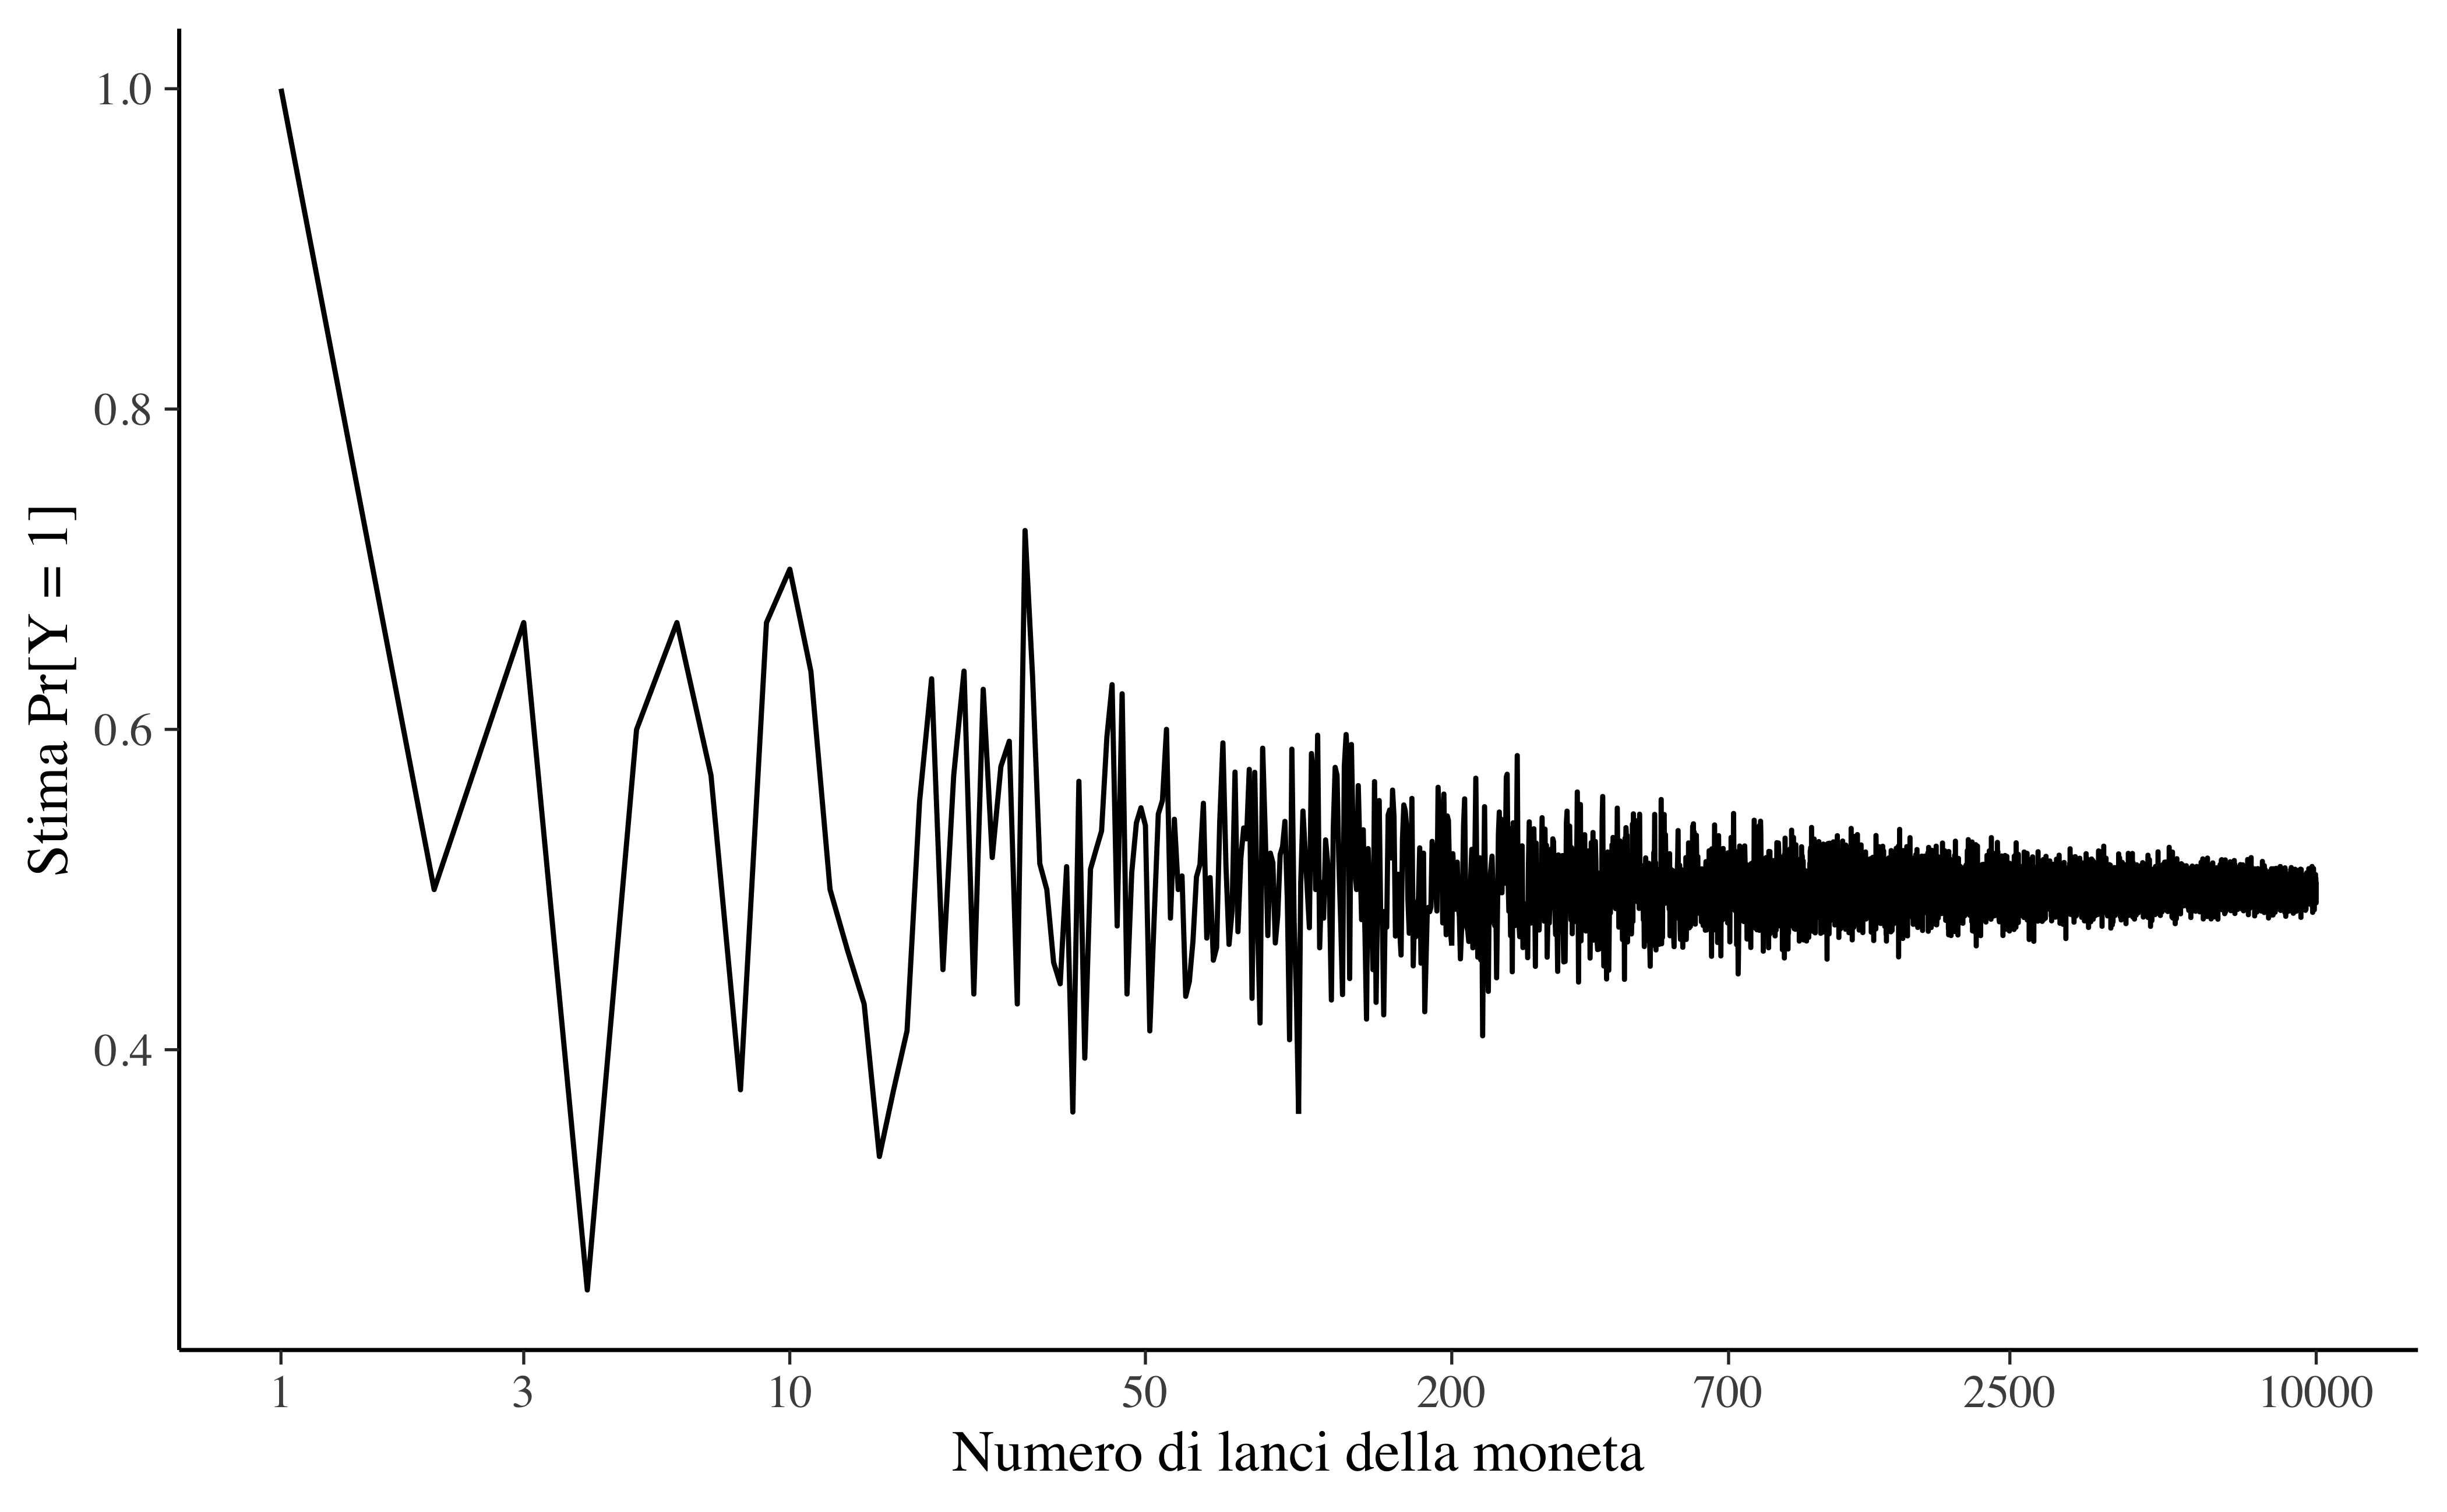
\includegraphics{ds4psy_files/figure-latex/legge-grandi-n-2-1} 

}

\caption{Stima della probabilità di successo in funzione del numero dei lanci di una moneta.}\label{fig:legge-grandi-n-2}
\end{figure}

La \emph{legge dei grandi numeri} ci dice che, all'aumentare del numero di ripetizioni dell'esperimento casuale, la media dei risultati ottenuti tende al valore atteso, man mano che vengono eseguite più prove. Nella figura \ref{fig:legge-grandi-n-2} vediamo infatti che, all'aumentare del numero \emph{M} di lanci della moneta, la stima di \(P(Y = 1)\) converge al valore 0.5.

\hypertarget{variabili-casuali-multiple}{%
\section{Variabili casuali multiple}\label{variabili-casuali-multiple}}

Le variabili casuali non esistono isolatamente. Abbiamo iniziato con una sola variabile casuale \(Y\) che rappresenta il risultato di un singolo, specifico lancio di una moneta equlibrata. Ma supponiamo ora di lanciare la moneta tre volte. I risultati di ciascuno dei tre lanci possono essere rappresentati da una diversa variabile casuale, ad esempio, \(Y_1 , Y_2 , Y_3\). Possiamo assumere che ogni lancio sia indipendente, ovvero che non dipenda dal risultato degli altri lanci. Per ciascuna di queste variabili \(Y_n\), con \(n \in 1:3\), abbiamo che \(P(Y_n =1)=0.5\) e \(P(Y_n =0)=0.5\).

È possibile combinare più variabili casuali usando le operazioni aritmetiche. Se \(Y_1 , Y_2, Y_3\) sono variabili casuali che rappresentano tre lanci di una moneta equilibrata (o un lancio di tre monete equilibrate), possiamo definire la somma di tali variabili casuali come

\[
Z = Y_1 + Y_2 + Y_3.
\]

Possiamo simulare i valori assunti dalla variabile casuale \emph{Z} simulando i valori di \(Y_1, Y_2, Y_3\) per poi sommarli.

\begin{Shaded}
\begin{Highlighting}[]
\NormalTok{y1 }\OtherTok{\textless{}{-}} \FunctionTok{rbinom}\NormalTok{(}\DecValTok{1}\NormalTok{, }\DecValTok{1}\NormalTok{, }\FloatTok{0.5}\NormalTok{)}
\NormalTok{y2 }\OtherTok{\textless{}{-}} \FunctionTok{rbinom}\NormalTok{(}\DecValTok{1}\NormalTok{, }\DecValTok{1}\NormalTok{, }\FloatTok{0.5}\NormalTok{)}
\NormalTok{y3 }\OtherTok{\textless{}{-}} \FunctionTok{rbinom}\NormalTok{(}\DecValTok{1}\NormalTok{, }\DecValTok{1}\NormalTok{, }\FloatTok{0.5}\NormalTok{)}
\FunctionTok{c}\NormalTok{(y1, y2, y3)}
\CommentTok{\#\textgreater{} [1] 1 0 1}
\NormalTok{z }\OtherTok{\textless{}{-}} \FunctionTok{sum}\NormalTok{(}\FunctionTok{c}\NormalTok{(y1, y2, y3))}
\FunctionTok{cat}\NormalTok{(}\StringTok{"z ="}\NormalTok{, z, }\StringTok{"}\SpecialCharTok{\textbackslash{}n}\StringTok{"}\NormalTok{)}
\CommentTok{\#\textgreater{} z = 2}
\end{Highlighting}
\end{Shaded}

ovvero,

\begin{Shaded}
\begin{Highlighting}[]
\NormalTok{y }\OtherTok{\textless{}{-}} \FunctionTok{rep}\NormalTok{(}\ConstantTok{NA}\NormalTok{, }\DecValTok{3}\NormalTok{)}
\ControlFlowTok{for}\NormalTok{ (i }\ControlFlowTok{in} \DecValTok{1}\SpecialCharTok{:}\DecValTok{3}\NormalTok{) \{}
\NormalTok{  y[i] }\OtherTok{\textless{}{-}} \FunctionTok{rbinom}\NormalTok{(}\DecValTok{1}\NormalTok{, }\DecValTok{1}\NormalTok{, }\FloatTok{0.5}\NormalTok{)}
\NormalTok{\}}
\NormalTok{y}
\CommentTok{\#\textgreater{} [1] 0 1 1}
\NormalTok{z }\OtherTok{\textless{}{-}} \FunctionTok{sum}\NormalTok{(y)}
\FunctionTok{cat}\NormalTok{(}\StringTok{"z ="}\NormalTok{, z, }\StringTok{"}\SpecialCharTok{\textbackslash{}n}\StringTok{"}\NormalTok{)}
\CommentTok{\#\textgreater{} z = 2}
\end{Highlighting}
\end{Shaded}

oppure, ancora più semplicemente:

\begin{Shaded}
\begin{Highlighting}[]
\NormalTok{y }\OtherTok{\textless{}{-}} \FunctionTok{rbinom}\NormalTok{(}\DecValTok{3}\NormalTok{, }\DecValTok{1}\NormalTok{, }\FloatTok{0.5}\NormalTok{)}
\NormalTok{y}
\CommentTok{\#\textgreater{} [1] 1 0 1}
\NormalTok{z }\OtherTok{\textless{}{-}} \FunctionTok{sum}\NormalTok{(y)}
\FunctionTok{cat}\NormalTok{(}\StringTok{"z ="}\NormalTok{, z, }\StringTok{"}\SpecialCharTok{\textbackslash{}n}\StringTok{"}\NormalTok{)}
\CommentTok{\#\textgreater{} z = 2}
\end{Highlighting}
\end{Shaded}

Possiamo ripetere questa simulazione \(M = 1e5\) volte:

\begin{Shaded}
\begin{Highlighting}[]
\NormalTok{M }\OtherTok{\textless{}{-}} \FloatTok{1e5}
\NormalTok{z }\OtherTok{\textless{}{-}} \FunctionTok{rep}\NormalTok{(}\ConstantTok{NA}\NormalTok{, M)}
\ControlFlowTok{for}\NormalTok{ (i }\ControlFlowTok{in} \DecValTok{1}\SpecialCharTok{:}\NormalTok{M) \{}
\NormalTok{  y }\OtherTok{\textless{}{-}} \FunctionTok{rbinom}\NormalTok{(}\DecValTok{3}\NormalTok{, }\DecValTok{1}\NormalTok{, }\FloatTok{0.5}\NormalTok{)}
\NormalTok{  z[i] }\OtherTok{\textless{}{-}} \FunctionTok{sum}\NormalTok{(y)}
\NormalTok{\}}
\end{Highlighting}
\end{Shaded}

e calcolare una stima della probabilità che la variabile casuale \(Z\) assuma i valori 0, 1, 2, 3:

\begin{Shaded}
\begin{Highlighting}[]
\FunctionTok{table}\NormalTok{(z) }\SpecialCharTok{/}\NormalTok{ M}
\CommentTok{\#\textgreater{} z}
\CommentTok{\#\textgreater{}      0      1      2      3 }
\CommentTok{\#\textgreater{} 0.1258 0.3750 0.3748 0.1244}
\end{Highlighting}
\end{Shaded}

Nel caso di 4 monete equilibrate, avremo:

\begin{Shaded}
\begin{Highlighting}[]
\NormalTok{M }\OtherTok{\textless{}{-}} \FloatTok{1e5}
\NormalTok{z }\OtherTok{\textless{}{-}} \FunctionTok{rep}\NormalTok{(}\ConstantTok{NA}\NormalTok{, M)}
\ControlFlowTok{for}\NormalTok{ (i }\ControlFlowTok{in} \DecValTok{1}\SpecialCharTok{:}\NormalTok{M) \{}
\NormalTok{  y }\OtherTok{\textless{}{-}} \FunctionTok{rbinom}\NormalTok{(}\DecValTok{4}\NormalTok{, }\DecValTok{1}\NormalTok{, }\FloatTok{0.5}\NormalTok{)}
\NormalTok{  z[i] }\OtherTok{\textless{}{-}} \FunctionTok{sum}\NormalTok{(y)}
\NormalTok{\}}
\FunctionTok{table}\NormalTok{(z) }\SpecialCharTok{/}\NormalTok{ M}
\CommentTok{\#\textgreater{} z}
\CommentTok{\#\textgreater{}       0       1       2       3       4 }
\CommentTok{\#\textgreater{} 0.06340 0.24917 0.37360 0.25022 0.06361}
\end{Highlighting}
\end{Shaded}

Una variabile casuale le cui modalità possono essere costituite solo da numeri interi è detta \emph{variabile casuale discreta}:

\[
\mathbb{Z} = \dots, -2, -1, 0, 1, 2, \dots
\]

\hypertarget{sec:fun-mass-prob}{%
\section{Funzione di massa di probabilità}\label{sec:fun-mass-prob}}

È conveniente avere una funzione che associa una probabilità a ciascun possibile valore di una variabile casuale. In generale, ciò è possibile se e solo se la variabile casuale è discreta, così com'è stata definita nel Paragrafo precedente. Ad esempio, se consideriamo \(Z = Y_1 + \dots + Y_4\) come il numero di risultati ``testa'' in 4 lanci della moneta, allora possiamo definire la seguente funzione:

\[
\begin{array}{rclll}
p_Z(0) & = & 1/16 & & \mathrm{TTTT}
\\
p_Z(1) & = & 4/16 & & \mathrm{HTTT, THTT, TTHT, TTTH}
\\
p_Z(2) & = & 6/16 & & \mathrm{HHTT, HTHT, HTTH, THHT, THTH, TTTH}
\\
p_Z(3) & = & 4/16 & & \mathrm{HHHT, HHTH, HTHH, THHH}
\\
p_Z(4) & = & 1/16 & & \mathrm{HHHH}
\end{array}
\]

Il lancio di quattro monete può produrre sedici possibili risultati. Dato che i lanci sono indipendenti e le monete sono equilibrate, ogni possibile risultato è ugualmente probabile. Nella tabella in alto, le sequenze dei risultati possibili del lancio delle 4 monete sono riportate nella colonna più a destra. Le probabilità si ottengono dividendo il numero di sequenze che producono lo stesso numero di eventi testa per il numero dei risultati possibili.

La funzione \(p_Z\) è stata costruita per associare a ciascun valore \(u\) della variabile casuale \(Z\) la probabilità dell'evento \(Z = u\). Convenzionalmente, queste probabilità sono scritte come

\[
P_Z(z) = \mbox{P}(Z = z).
\]

La parte a destra dell'uguale si può leggere come: ``la probabilità che la variabile casuale \(Z\) assuma il valore \(z\)''. Una funzione definita come sopra è detta \emph{funzione di massa di probabilità} della variabile casuale \(Z\). Ad ogni variabile casuale discreta è associata un'unica funzione di massa di probabilità.

Una rappresentazione grafica della stima della funzione di massa di probabilità per l'esperimento casuale del lancio di quattro monete equilibrate è fornita nella figura \ref{fig:barplot-mdf-4coins}.

\begin{Shaded}
\begin{Highlighting}[]
\FunctionTok{set.seed}\NormalTok{(}\DecValTok{1234}\NormalTok{)}
\NormalTok{M }\OtherTok{\textless{}{-}} \FloatTok{1e5}
\NormalTok{nflips }\OtherTok{\textless{}{-}} \DecValTok{4}
\NormalTok{u }\OtherTok{\textless{}{-}} \FunctionTok{rbinom}\NormalTok{(M, nflips, }\FloatTok{0.5}\NormalTok{)}
\NormalTok{x }\OtherTok{\textless{}{-}} \DecValTok{0}\SpecialCharTok{:}\NormalTok{nflips}
\NormalTok{y }\OtherTok{\textless{}{-}} \FunctionTok{rep}\NormalTok{(}\ConstantTok{NA}\NormalTok{, nflips }\SpecialCharTok{+} \DecValTok{1}\NormalTok{)}
\ControlFlowTok{for}\NormalTok{ (n }\ControlFlowTok{in} \DecValTok{0}\SpecialCharTok{:}\NormalTok{nflips) \{}
\NormalTok{  y[n }\SpecialCharTok{+} \DecValTok{1}\NormalTok{] }\OtherTok{\textless{}{-}} \FunctionTok{sum}\NormalTok{(u }\SpecialCharTok{==}\NormalTok{ n) }\SpecialCharTok{/}\NormalTok{ M}
\NormalTok{\}}
\NormalTok{bar\_plot }\OtherTok{\textless{}{-}}
  \FunctionTok{data.frame}\NormalTok{(}\AttributeTok{Z =}\NormalTok{ x, }\AttributeTok{count =}\NormalTok{ y) }\SpecialCharTok{\%\textgreater{}\%}
  \FunctionTok{ggplot}\NormalTok{(}\FunctionTok{aes}\NormalTok{(}\AttributeTok{x =}\NormalTok{ Z, }\AttributeTok{y =}\NormalTok{ count)) }\SpecialCharTok{+}
  \FunctionTok{geom\_bar}\NormalTok{(}\AttributeTok{stat =} \StringTok{"identity"}\NormalTok{) }\SpecialCharTok{+}
  \FunctionTok{scale\_x\_continuous}\NormalTok{(}
    \AttributeTok{breaks =} \DecValTok{0}\SpecialCharTok{:}\DecValTok{4}\NormalTok{,}
    \AttributeTok{labels =} \FunctionTok{c}\NormalTok{(}\DecValTok{0}\NormalTok{, }\DecValTok{1}\NormalTok{, }\DecValTok{2}\NormalTok{, }\DecValTok{3}\NormalTok{, }\DecValTok{4}\NormalTok{)}
\NormalTok{  ) }\SpecialCharTok{+}
  \FunctionTok{labs}\NormalTok{(}
    \AttributeTok{y =} \StringTok{"Probabilità stimata P(Z = z)"}
\NormalTok{  )}
\NormalTok{bar\_plot}
\end{Highlighting}
\end{Shaded}

\begin{figure}

{\centering 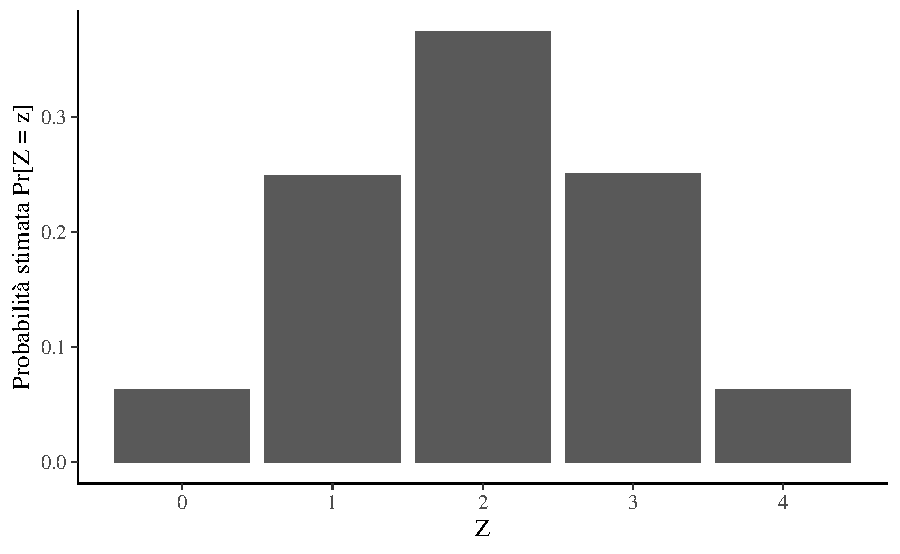
\includegraphics{ds4psy_files/figure-latex/barplot-mdf-4coins-1} 

}

\caption{Grafico di $M = 100,000$ simulazioni della funzione di massa di probabilità di una variabile casuale definita come il numero di teste in quattro lanci di una moneta equilibrata.}\label{fig:barplot-mdf-4coins}
\end{figure}

Se \(A\) è un sottoinsieme della variabile casuale \(Z\), allora denotiamo con \(P_{z}(A)\) la probabilità assegnata ad \(A\) dalla distribuzione \(P_{z}\). Mediante una distribuzione di probabilità \(P_{z}\) è dunque possibile determinare la probabilità di ciascun sottoinsieme \(A \subset Z\) come

\begin{equation}
P_{z}(A) = \sum_{z \in A} P_{z}(Z).
\end{equation}

Una funzione di massa di probabilità soddisfa le proprietà \(0 \leq P(X=x) \leq 1\) e \(\sum_{x \in X} P(x) = 1\).

\begin{example}
Nel caso dell'esempio discusso nel Paragrafo \ref{sec:fun-mass-prob}, la probabilità che la variabile casuale \(Z\) sia un numero dispari è

\[
P(\text{Z è un numero dispari}) = P_{z}(Z = 1) + P_{z}(Z = 3) = \frac{4}{16} + \frac{4}{16} = \frac{1}{2}.
\]
\end{example}

\hypertarget{funzione-di-ripartizione}{%
\subsection{Funzione di ripartizione}\label{funzione-di-ripartizione}}

Data una variabile casuale discreta \(X\) possiamo calcolare la probabilità che \(X\) non superi un certo valore \(x\), ossia la sua \emph{funzione di ripartizione}. Poichè \(X\) assume valori discreti possiamo cumulare le probabilità mediante una somma:

\begin{equation}
F(x_k) = P(X \leq x_k) = \sum_{x \leq x_k} P(x).
\end{equation}

\hypertarget{commenti-e-considerazioni-finali}{%
\section*{Commenti e considerazioni finali}\label{commenti-e-considerazioni-finali}}


In questo capitolo abbiamo visto come si costruisce lo spazio campione di un esperimento casuale, quali sono le proprietà di base della probabilità e come si assegnano le probabilità agli eventi definiti sopra uno spazio campione discreto. Abbiamo anche introdotto le nozioni di variabile casuale, ovvero di una variabile che assume i suoi valori in maniera casuale. Abbiamo descritto il modo di specificare la probabilità con cui sono una variabile casuale assume i suoi differenti valori, ovvero la funzione di ripartizione \(F(X) = P(X < x)\) e la funzione di massa di probabilità.

\hypertarget{exp-val-and-variance-rv}{%
\chapter{Valore atteso e varianza}\label{exp-val-and-variance-rv}}

Spesso risulta utile fornire una rappresentazione sintetica della distribuzione di una variabile casuale attraverso degli indicatori caratteristici piuttosto che fare riferimento ad una sua rappresentazione completa mediante la funzione di ripartizione, o la funzione di massa o di densità di probabilità. Una descrizione più sintetica di una variabile casuale, tramite pochi valori, ci consente di cogliere le caratteristiche essenziali della distribuzione, quali: la posizione, cioè il baricentro della distribuzione di probabilità; la variabilità, cioè la dispersione della distribuzione di probabilità attorno ad un centro; la forma della distribuzione di probabilità, considerando la simmetria e la curtosi (pesantezza delle code). In questo Capitolo introdurremo quegli indici sintetici che descrivono il centro di una distribuzione di probabilità e la sua variabilità.

\hypertarget{valore-atteso}{%
\section{Valore atteso}\label{valore-atteso}}

Quando vogliamo conoscere il comportamento tipico di una variabile casuale spesso vogliamo sapere qual è il suo ``valore tipico''. La nozione di ``valore tipico'', tuttavia, è ambigua. Infatti, essa può essere definita in almeno tre modi diversi:

\begin{itemize}
\tightlist
\item
  la \emph{media} (somma dei valori divisa per il numero dei valori),
\item
  la \emph{mediana} (il valore centrale della distribuzione, quando la variabile è ordinata in senso crescente o decrescente),
\item
  la \emph{moda} (il valore che ricorre più spesso).
\end{itemize}

Per esempio, la media di \(\{3, 1, 4, 1, 5\}\) è \(\frac{3+1+4+1+5}{5} = 2.8\), la mediana è \(3\) e la moda è \(1\). Tuttavia, la teoria delle probabilità si occupa di variabili casuali piuttosto che di sequenze di numeri. Diventa dunque necessario precisare che cosa intendiamo per ``valore tipico'' quando facciamo riferimento alle variabili casuali. Giungiamo così alla seguente definizione.

\begin{definition}
Sia \(Y\) è una variabile casuale discreta che assume i valori \(y_1, \dots, y_n\) con distribuzione \(p(y)\), ossia

\[
P(Y = y_i) = p(y_i),
\]

per definizione il \emph{valore atteso} di \(Y\), \(\E(Y)\), è

\begin{equation}
\E(Y) = \sum_{i=1}^n y_i \cdot p(y_i).
\label{eq:expval-discr}
\end{equation}
\end{definition}

A parole: il valore atteso (o speranza matematica, o aspettazione, o valor medio) di una variabile casuale è definito come la somma di tutti i valori che la variabile casuale può prendere, ciascuno pesato dalla probabilità con cui il valore è preso.

\begin{exercise}
Calcoliamo il valore atteso della variabile casuale \(Y\) corrispondente al lancio di una moneta equilibrata (testa: \emph{Y} = 1; croce: \emph{Y} = 0).

\[
\E(Y) = \sum_{i=1}^{2} y_i \cdot P(y_i) = 0 \cdot \frac{1}{5} + 1 \cdot \frac{1}{5} = 0.5.
\]
\end{exercise}

\begin{exercise}
Supponiamo ora che \emph{Y} sia il risultato del lancio di un dado equilibrato. Il valore atteso di \emph{Y} diventa:

\[
\E(Y) = \sum_{i=1}^{6} y_i \cdot P(y_i) = 1 \cdot \frac{1}{6} + 2 \cdot \frac{1}{6} + \dots + 6 \cdot \frac{1}{6} = \frac{21}{6} = 3.5.
\]
\end{exercise}

\hypertarget{interpretazione}{%
\subsection{Interpretazione}\label{interpretazione}}

Che interpretazione può essere assegnata alla nozione di valore atteso? Bruno de Finetti adottò lo stesso termine di \emph{previsione} (e lo stesso simbolo) tanto per la probabilità che per la speranza matematica. Si può pertanto dire che, dal punto di vista bayesiano, la speranza matematica è l'estensione naturale della nozione di probabilità soggettiva.

\hypertarget{proprietuxe0-del-valore-atteso}{%
\subsection{Proprietà del valore atteso}\label{proprietuxe0-del-valore-atteso}}

La proprietà più importante del valore atteso è la linearità: il valore atteso di una somma di variabili casuali è uguale alla somma dei lori rispettivi valori attesi:

\begin{equation}
\E(X + Y) = \E(X) + \E(Y).
\label{eq:prop-expval-linearity}
\end{equation}

La \eqref{eq:prop-expval-linearity} sembra ragionevole quando \(X\) e \(Y\) sono indipendenti, ma è anche vera quando \(X\) e \(Y\) sono associati. Abbiamo anche che

\begin{equation}
\E(cY) = c \E(Y).
\label{eq:prop-expval-const}
\end{equation}

La \eqref{eq:prop-expval-const} ci dice che possiamo estrarre una costante dall'operatore di valore atteso. Tale proprietà si estende a qualunque numero di variabili casuali. Infine, se due variabili casuali \(X\) e \(Y\) sono indipendenti, abbiamo che

\begin{equation}
\E(X Y) = \E(X) \E(Y). 
\label{eq:expval-prod-ind-rv}
\end{equation}

\begin{exercise}
Si considerino le seguenti variabili casuali: \(Y\), ovvero il numero che si ottiene dal lancio di un dado equilibrato, e \(Y\), il numero di teste prodotto dal lancio di una moneta equilibrata. Poniamoci il problema di trovare il valore atteso di \(X+Y\).

Per risolvere il problema iniziamo a costruire lo spazio campionario dell'esperimento casuale consistente nel lancio di un dado e di una moneta.

\begin{longtable}[]{@{}ccccccc@{}}
\toprule
\(x/ y\) & 1 & 2 & 3 & 4 & 5 & 6 \\
\midrule
\endhead
0 & (0, 1) & (0, 2) & (0, 3) & (0, 4) & (0, 5) & (0, 6) \\
1 & (1, 1) & (1, 2) & (1, 3) & (1, 4) & (1, 5) & (1, 6) \\
\bottomrule
\end{longtable}

\noindent ovvero

\begin{longtable}[]{@{}ccccccc@{}}
\toprule
\(x/ y\) & 1 & 2 & 3 & 4 & 5 & 6 \\
\midrule
\endhead
0 & 1 & 2 & 3 & 4 & 5 & 6 \\
1 & 2 & 3 & 4 & 5 & 6 & 7 \\
\bottomrule
\end{longtable}

\noindent Il risultato del lancio del dado è indipendente dal risultato del lancio della moneta. Pertanto, ciascun evento elementare dello spazio campionario avrà la stessa probabilità di verificarsi, ovvero \(Pr(\omega) = \frac{1}{12}\). Il valore atteso di \(X+Y\) è dunque uguale a:

\[
\E(X+Y) = 1 \cdot \frac{1}{12} + 2 \cdot \frac{1}{12} + \dots + 7 \cdot \frac{1}{12} = 4.0.
\]

Lo stesso risultato si ottiene nel modo seguente:

\[
\E(X+Y) = \E(X) + E(Y) = 3.5 + 0.5 = 4.0.
\]
\end{exercise}

\begin{exercise}
Si considerino le variabili casuali \(X\) e \(Y\) definite nel caso del lancio di tre monete equilibrate, dove \(X\) conta il numero delle teste nei tre lanci e \(Y\) conta il numero delle teste al primo lancio. Si calcoli il valore atteso del prodotto delle variabili casuali \(X\) e \(Y\).

La distribuzione di probabilità congiunta \(P(X, Y)\) è fornita nella tabella seguente.

\begin{longtable}[]{@{}cccc@{}}
\toprule
\(x/ y\) & 0 & 1 & \(p(Y)\) \\
\midrule
\endhead
0 & 1/8 & 0 & 1/8 \\
1 & 2/8 & 1/8 & 3/8 \\
2 & 1/8 & 2/8 & 3/8 \\
3 & 0 & 1/8 & 1/8 \\
\(p(y)\) & 4/8 & 4/8 & 1.0 \\
\bottomrule
\end{longtable}

\noindent Il calcolo del valore atteso di \(XY\) si riduce a

\[
\E(XY) = 1 \cdot \frac{1}{8} + 2 \cdot \frac{2}{8} + 3 \cdot \frac{1}{8} = 1.0.
\]

Si noti che le variabili casuali \(Y\) e \(Y\) non sono indipendenti. Dunque non possiamo usare la proprietà \ref{thm:prodindrv}. Infatti, il valore atteso di \(X\) è

\[
\E(X) = 1 \cdot \frac{3}{8} + 2 \cdot \frac{3}{8} + 3 \cdot \frac{1}{8} = 1.5
\]

e il valore atteso di \(Y\) è

\[
\E(Y) = 0 \cdot \frac{4}{8} + 1 \cdot \frac{4}{8} = 0.5.
\] Dunque

\[
1.5 \cdot 0.5 \neq 1.0.
\]
\end{exercise}

\hypertarget{variabili-casuali-continue}{%
\subsection{Variabili casuali continue}\label{variabili-casuali-continue}}

Nel caso di una variabile casuale continua \(Y\) il valore atteso diventa:

\begin{equation}
\E(Y) = \int_{-\infty}^{+\infty} y p(y) \,\operatorname {d}\!y
\label{eq:def-ev-rv-cont}
\end{equation}

Anche in questo caso il valore atteso è una media ponderata della \(y\), nella quale ciascun possibile valore \(y\) è ponderato per il corrispondente valore della densità \(p(y)\). Possiamo leggere l'integrale pensando che \(y\) rappresenti l'ampiezza delle barre infinitamente strette di un istogramma, con la densità \(p(y)\) che corrisponde all'altezza di tali barre e la notazione \(\int_{-\infty}^{+\infty}\) che corrisponde ad una somma.

Un'altra misura di tendenza centrale delle variabili casuali continue è la moda. La moda della \(Y\) individua il valore \(y\) più plausibile, ovvero il valore \(y\) che massimizza la funzione di densità \(p(y)\):

\begin{equation}
\Mo(Y) = \argmax_y p(y).
\label{eq:def-mode}
\end{equation}

\hypertarget{varianza}{%
\section{Varianza}\label{varianza}}

La seconda più importante proprietà di una variabile casuale, dopo che conosciamo il suo valore atteso, è la \emph{varianza}.

\begin{definition}
Se \(Y\) è una variabile casuale discreta con distribuzione \(p(y)\), per definizione la varianza di \(Y\), \(\mathbb{V}(Y)\), è

\begin{equation}
\mathbb{V}(Y) = \E\Big[\big(Y - \E(Y)\big)^2\Big].
\label{eq:def-var-rv}
\end{equation}
\end{definition}

A parole: la varianza è la deviazione media quadratica della variabile dalla sua media.\footnote{Data una variabile casuale \(Y\) con valore atteso \(\E(Y)\), le ``distanze'' tra i valori di \(Y\) e il valore atteso \(\E(Y)\) definiscono la variabile casuale \(Y - \E(Y)\) chiamata \emph{scarto}, oppure \emph{deviazione} oppure \emph{variabile casuale centrata}. La variabile \(Y - \E(Y)\) equivale ad una traslazione di sistema di riferimento che porta il valore atteso nell'origine degli assi. Si può dimostrare facilmente che il valore atteso della variabile scarto \(Y - \E(Y)\) vale zero, dunque la media di tale variabile non può essere usata per quantificare la ``dispersione'' dei valori di \(Y\) relativamente al suo valore medio. Occorre rendere sempre positivi i valori di \(Y - \E(Y)\) e tale risultato viene ottenuto considerando la variabile casuale \(\left(Y - \E(Y)\right)^2\).} Se denotiamo \(\E(Y) = \mu\), la varianza \(\mathbb{V}(Y)\) diventa il valore atteso di \((Y - \mu)^2\).

\begin{exercise}
Posta \(S\) uguale alla somma dei punti ottenuti nel lancio di due dadi equilibrati, poniamoci il problema di calcolare la varianza di \(S\).

La variabile casuale \(S\) ha la seguente distribuzione di probabilità:

\begin{longtable}[]{@{}cccccccccccc@{}}
\toprule
\(s\) & 2 & 3 & 4 & 5 & 6 & 7 & 8 & 9 & 10 & 11 & 12 \\
\midrule
\endhead
\(P(S = s)\) & \(\frac{1}{36}\) & \(\frac{2}{36}\) & \(\frac{3}{36}\) & \(\frac{4}{36}\) & \(\frac{5}{36}\) & \(\frac{6}{36}\) & \(\frac{5}{36}\) & \(\frac{4}{36}\) & \(\frac{3}{36}\) & \(\frac{2}{36}\) & \(\frac{1}{36}\) \\
\bottomrule
\end{longtable}

\noindent Essendo \(\E(S) = 7\), la varianza diventa

\begin{align}
\mathbb{V}(S) &= \sum \left(S- \mathbb{E}(S)\right)^2 \cdot P(S) \notag\\
&= (2 - 7)^2 \cdot 0.0278 + (3-7)^2 \cdot 0.0556 + \dots + (12 - 7)^2 \cdot 0.0278 \notag\\
&= 5.8333.\notag
\end{align}
\end{exercise}

\hypertarget{formula-alternativa-per-la-varianza}{%
\subsection{Formula alternativa per la varianza}\label{formula-alternativa-per-la-varianza}}

C'è un modo più semplice per calcolare la varianza:

\begin{align}
\E\Big[\big(X - \E(Y)\big)^2\Big] &= \E\big(X^2 - 2X\E(Y) + \E(Y)^2\big)\notag\\
&= \E(Y^2) - 2\E(Y)\E(Y) + \E(Y)^2,\notag
\end{align}

dato che \(\E(Y)\) è una costante; pertanto

\begin{equation}
\mathbb{V}(Y) = \E(Y^2) - \big(\E(Y) \big)^2.
\label{eq:def-alt-var-rv}
\end{equation}

A parole: la varianza è la media dei quadrati meno il quadrato della media.

\begin{exercise}
Consideriamo la variabile casuale \(Y\) che corrisponde al numero di teste che si osservano nel lancio di una moneta truccata con probabilità di testa uguale a 0.8. Il valore atteso di \(Y\) è

\[
\E(Y) = 0 \cdot 0.2 + 1 \cdot 0.8 = 0.8.
\] Usando la formula tradizionale della varianza otteniamo:

\[
\mathbb{V}(Y) = (0 - 0.8)^2 \cdot 0.2 + (1 - 0.8)^2 \cdot 0.8 = 0.16.
\] Lo stesso risultato si trova con la formula alternativa della varianza. Il valore atteso di \(Y^2\) è

\[
\E(Y^2) = 0^2 \cdot 0.2 + 1^2 * 0.8 = 0.8.
\] e la varianza diventa

\[
\mathbb{V}(Y) = \E(Y^2) - \big(\E(Y) \big)^2 = 0.8 - 0.8^2 = 0.16.
\]
\end{exercise}

\hypertarget{variabili-casuali-continue-1}{%
\subsection{Variabili casuali continue}\label{variabili-casuali-continue-1}}

Nel caso di una variabile casuale continua \(Y\), la varianza diventa:

\begin{equation}
\mathbb{V}(Y) = \int_{-\infty}^{+\infty} \large[y - \E(Y)\large]^2 p(y) \,\operatorname {d}\!y
\label{eq:def-var-rv-cont}
\end{equation}

Come nel caso discreto, la varianza di una v.c. continua \(y\) misura approssimativamente la distanza al quadrato tipica o prevista dei possibili valori \(y\) dalla loro media.

\hypertarget{deviazione-standard}{%
\section{Deviazione standard}\label{deviazione-standard}}

Quando lavoriamo con le varianze, i termini sono innalzati al quadrato e quindi i numeri possono diventare molto grandi (o molto piccoli). Per trasformare nuovamente i valori nell'unità di misura della scala originaria si prende la radice quadrata. Il valore risultante viene chiamato \emph{deviazione standard} e solitamente è denotato dalla lettera greca \(\sigma\).

\begin{definition}
Si definisce scarto quadratico medio (o deviazione standard o scarto tipo) la radice quadrata della varianza:

\begin{equation}
\sigma_Y = \sqrt{\mathbb{V}(Y)}.
\label{eq:def-sd}
\end{equation}
\end{definition}

Interpretiamo la deviazione standard di una variabile casuale come nella statistica descrittiva: misura approssimativamente la distanza tipica o prevista dei possibili valori \(y\) dalla loro media.

\begin{exercise}
Per i dadi equilibrati dell'esempio precedente, la deviazione standard della variabile casuale \(S\) è uguale a \(\sqrt{5.833} = 2.415\).
\end{exercise}

\hypertarget{standardizzazione}{%
\section{Standardizzazione}\label{standardizzazione}}

\begin{definition}
Data una variabile casuale \(Y\), si dice variabile standardizzata di \(Y\) l'espressione

\begin{equation}
Z = \frac{Y - \E(Y)}{\sigma_Y}.
\label{eq:standardization}
\end{equation}
\end{definition}

Solitamente, una variabile standardizzata viene denotata con la lettera \(Z\).

\hypertarget{momenti-di-variabili-casuali}{%
\section{Momenti di variabili casuali}\label{momenti-di-variabili-casuali}}

\begin{definition}
Si chiama \emph{momento} di ordine \(q\) di una v.c. \(X\), dotata di densità \(p(x)\), la quantità

\begin{equation}
\E(X^q) = \int_{-\infty}^{+\infty} x^q p(x) \; dx.
\end{equation}

Se \(X\) è una v.c. discreta, i suoi momenti valgono:

\begin{equation}
\E(X^q) = \sum_i x_i^q p(x_i).
\end{equation}
\end{definition}

I momenti sono importanti parametri indicatori di certe proprietà di \(X\). I più noti sono senza dubbio quelli per \(q = 1\) e \(q = 2\). Il momento del primo ordine corrisponde al valore atteso di \(X\). Spesso i momenti di ordine superiore al primo vengono calcolati rispetto al valor medio di \(X\), operando una traslazione \(x_0 = x − \E(X)\) che individua lo scarto dalla media. Ne deriva che il momento centrale di ordine 2 corrisponde alla varianza.

\hypertarget{covarianza}{%
\section{Covarianza}\label{covarianza}}

La covarianza quantifica la tendenza delle variabili aleatorie \(X\) e \(Y\) a ``variare assieme'\,'. Per esempio, l'altezza e il peso delle giraffe producono una covarianza positiva perché all'aumentare di una di queste due quantità tende ad aumentare anche l'altra. La covarianza misura la forza e la direzione del legame lineare tra due variabili aleatorie \(X\) ed \(Y\). Si utilizza la notazione \(\mbox{Cov}(X,Y)=\sigma_{xy}\).

\begin{definition}
Date due variabili aleatorie \(X\), \(Y\), chiamiamo covarianza tra \(X\) ed \(Y\) il numero

\begin{equation}
\mbox{Cov}(X,Y) = \mathbb{E}\Bigl(\bigl(X - \mathbb{E}(X)\bigr) \bigl(Y - \mathbb{E}(Y)\bigr)\Bigr),
\end{equation}

dove \(\mathbb{E}(X)\) e \(\mathbb{E}(Y)\) sono i valori attesi di \(X\) ed \(Y\).
\end{definition}

In maniera esplicita,

\begin{equation}
\mbox{Cov}(X,Y) = \sum_{(x,y) \in \Omega} (x - \mu_X) (y - \mu_Y) f(x, y).
\label{eq:cov_def}
\end{equation}

La definizione è analoga, algebricamente, a quella di varianza e risulta infatti

\begin{equation}
\mathbb{V}(x) = cov(X, X)
\end{equation}

e

\begin{equation}
\mbox{Cov}(X,Y) = \mathbb{E}(XY) - \mathbb{E}(Y)\mathbb{E}(X).
\label{eq:cov_vc_alt}
\end{equation}

\begin{proof}
La proprietà precedente si dimostra nel modo seguente:

\begin{align}
\mbox{Cov}(X,Y) &= \mathbb{E}\Bigl(\bigl(X-\mathbb{E}(X)\bigr) \bigl(Y-\mathbb{E}(Y)\bigr)\Bigr)\notag\\
          %&= \mathbb{E}(XY) - \mathbb{E}(Y)X -\mathbb{E}(X)Y + \mathbb{E}(X)\mathbb{E}(Y) )\notag\\
          &= \mathbb{E}(XY) - \mathbb{E}(Y)\mathbb{E}(X) - \mathbb{E}(X)\mathbb{E}(Y) + \mathbb{E}(X)\mathbb{E}(Y)\notag\\
          &= \mathbb{E}(XY) - \mathbb{E}(Y)\mathbb{E}(X)\notag.
\end{align}
\end{proof}

\begin{exercise}
Consideriamo le variabili casuali definite nell'Esercizio 2.4. Si calcoli la covarianza di \(X\) e \(Y\).

Abbiamo che \(\mu_X = 1.5\) e \(\mu_Y = 0.5\). Ne segue che la covarianza di \(X\) e \(Y\) è:

\begin{equation}
\begin{split}
\mbox{Cov}(X,Y) &= \sum_{(x,y) \in\ \Omega} (x - \mu_X) (y - \mu_Y) f(x, y)\\
&= (0-1.5)(0-0.5)\cdot \frac{1}{8} + (0-1.5)(1-0.5) \cdot 0 \\
   &\hskip0.05\textwidth\relax + (1-1.5)(0-0.5)\cdot \frac{2}{8} + (1-1.5)(1-0.5) \cdot \frac{1}{8} \\
    &\hskip0.05\textwidth\relax + (2-1.5)(0-0.5) \cdot \frac{1}{8} + (2-1.5)(1-0.5) \cdot \frac{2}{8} \\
   &\hskip0.05\textwidth\relax + (3-1.5)(0-0.5) \cdot 0 +  (3-1.5)(1-0.5)\cdot\frac{1}{8} \\
   &= \frac{1}{4}. \notag
 \end{split}
\end{equation}

Lo stesso risultato può essere trovato nel modo seguente. Iniziamo a calcolare il valore atteso del prodotto \(XY\):

\[
\mathbb{E}(XY) = 0 \cdot\frac{4}{8} + 1 \cdot\frac{1}{8} + 2 \cdot\frac{2}{8} + 3 \cdot\frac{1}{8} = 1.0.
\]

Dunque, la covarianza tra \(X\) e \(Y\) diventa

\begin{align}
\mbox{Cov}(X,Y) &= \mathbb{E}(XY) - \mathbb{E}(X)\mathbb{E}(Y)\notag\\
 &= 1 -  1.5\cdot 0.5 \notag\\
 &= 0.25.\notag
\end{align}
\end{exercise}

\hypertarget{correlazione}{%
\section{Correlazione}\label{correlazione}}

La covarianza dipende dall'unità di misura delle due variabili e quindi non consente di stabilire l'intensità della relazione. Una misura standardizzata della relazione che intercorre fra due variabili è invece rappresentata dalla correlazione. La correlazione si ottiene dividendo la covarianza per le deviazioni standard delle due variabili aleatorie.

Il coefficiente di correlazione tra \(X\) ed \(Y\) è il numero definito da

\begin{equation}
\rho(X,Y) =\frac{\mbox{Cov}(X,Y)}{\sqrt{\mathcal{V}(X)\mathcal{V}(Y)}}.
\end{equation}

Si può anche scrivere \(\rho_{X,Y}\) al posto di \(\rho(X,Y)\).

Il coefficiente di correlazione \(\rho_{xy}\) è un numero puro, cioè non dipende dall'unità di misura delle variabili, e assume valori compresi tra -1 e +1.

\hypertarget{proprietuxe0}{%
\section{Proprietà}\label{proprietuxe0}}

\begin{itemize}
\tightlist
\item
  La covarianza tra una variabile aleatoria \(X\) e una costante \(c\) è nulla:
\end{itemize}

\begin{equation}
\mbox{Cov}(c,X) = 0,
\end{equation}

\begin{itemize}
\tightlist
\item
  la covarianza è simmetrica:
\end{itemize}

\begin{equation}
\mbox{Cov}(X,Y) = \mbox{Cov}(Y,X),
\end{equation}

\begin{itemize}
\tightlist
\item
  vale
\end{itemize}

\begin{equation}
 -1 \leq \rho(X,Y) \leq 1,
\end{equation}

\begin{itemize}
\tightlist
\item
  la correlazione non dipende dall'unità di misura:
\end{itemize}

\begin{equation}
 \rho(aX, bY) = \rho(X,Y), \qquad \forall a, b > 0,
\end{equation}

\begin{itemize}
\tightlist
\item
  se \(Y = a + bX\) è una funzione lineare di \(X\) con costanti \(a\) e \(b\), allora \(\rho(X,Y) = \pm 1\), a seconda del segno di \(b\),
\item
  la covarianza tra \(X\) e \(Y\), ciascuna moltiplicata per una costante, è uguale al prodotto delle costanti per la covarianza tra \(X\) e \(Y\):
\end{itemize}

\begin{equation}
\mbox{Cov}(aX,bY) = ab \;\mbox{Cov}(X,Y), \qquad \forall a,b \in \Real,
\end{equation}

\begin{itemize}
\tightlist
\item
  vale
\end{itemize}

\begin{equation}
\mathbb{V}(X \pm Y) = \mathbb{V}(X) + \mathbb{V}(Y) \pm 2 \cdot \mbox{Cov}(X,Y),
\end{equation}

\begin{itemize}
\tightlist
\item
  vale
\end{itemize}

\begin{equation}
\mbox{Cov}(X + Y, Z) = \mbox{Cov}(X,Z) + \mbox{Cov}(Y,Z),
\end{equation}

\begin{itemize}
\tightlist
\item
  per una sequenza di variabili aleatorie \(X_1, \dots, X_n\), si ha
\end{itemize}

\begin{equation}
 \mathbb{V}\left( \sum_{i=1}^n X_i\right) = \sum_{i=1}^n
 \mathbb{V}(X_i) + 2\sum_{i,j: i<j}cov(X_i, X_j),
\end{equation}

\begin{itemize}
\tightlist
\item
  vale
\end{itemize}

\begin{equation}
\mbox{Cov}\left(\sum_{i=1}^n a_i X_i, \sum_{j=1}^m b_jY_j\right) = \sum_{i=1}^n \sum_{j=1}^m a_j b_j\mbox{Cov}(X_j, Y_j),
\end{equation}

\begin{itemize}
\tightlist
\item
  se \(X_1, X_2, \dots, X_n\) sono indipendenti, allora
\end{itemize}

\begin{equation}
\mbox{Cov}\left(\sum_{i=1}^n a_i X_i, \sum_{j=1}^n b_jX_j\right) = \sum_{i=1}^n a_i b_i \mathbb{V}(X_i).
\end{equation}

\hypertarget{incorrelazione}{%
\subsection{Incorrelazione}\label{incorrelazione}}

Si dice che \(X\) ed \(Y\) sono incorrelate, o linermente indipendenti, se la loro covarianza è nulla,

\begin{equation}
\sigma_{XY} = \mathbb{E} \big[(X - \mu_X) (y-\mu_u) \big] = 0,
\end{equation}

che si può anche scrivere come

\begin{equation}
\rho_{XY} = 0, \quad \mathbb{E}(XY) = \mathbb{E}(X) \mathbb{E}(Y).
\end{equation}

Si introduce così un secondo tipo di indipendenza, più debole, dopo quello di indipendenza stocastica. Viceversa, però, se \(\mbox{Cov}(X, Y) = 0\), non è detto che \(X\) ed \(Y\) siano indipendenti.

\begin{exercise}
Siano \(X\) e \(Y\) due variabili aleatorie discrete avente una distribuzione di massa di probabilità congiunta pari a

\[
f_{XY}(x,y) = \frac{1}{4} \quad (x,y) \in \{(0,0), (1,1), (1, -1), (2,0) \}
\]

e zero altrimenti. Si calcoli la covarianza \(\rho_{XY}\). Le due variabili aleatorie \(X\) e \(Y\) sono mutuamente indipendenti?

La distribuzione marginale della \(X\) è

\[
\begin{cases}
X = 0, \quad  P_X = 1/4, \\
X = 1, \quad P_X = 2/4, \\
X = 2, \quad P_X = 1/4.
\end{cases}
\]

\[
\mathbb{E}(X) = 0 \frac{1}{4} + 1 \frac{2}{4} + 2 \frac{1}{4} = 1.
\]

\[
\mathbb{E}(X^2) = 0^2 \frac{1}{4} + 1^2 \frac{2}{4} + 2^2 \frac{1}{4} = \frac{3}{2}.
\]

\[
\mathbb{V}(X) = \frac{3}{2} - 1^2 = \frac{1}{2}.
\]

La distribuzione marginale della \(Y\) è

\[
\begin{cases}
Y = -1, \quad  P_Y = 1/4, \\
Y = 0, \quad P_Y = 2/4, \\
Y = 1, \quad P_Y = 1/4.
\end{cases}
\]

\[
\mathbb{E}(Y) = 0 \frac{2}{4} + 1 \frac{1}{4} + (-1) \frac{1}{4} = 0.
\]

\[
\mathbb{E}(Y^2) = 0^2 \frac{2}{4} + 1^2 \frac{1}{4} + (-1)^2 \frac{1}{4} = \frac{1}{2}.
\]

\[
\mathbb{V}(X) = \frac{1}{2} - 0^2 = \frac{1}{2}.
\]

Calcoliamo ora la covarianza tra \(X\) e \(Y\):

\[
\mathbb{E}(XY) = \sum_x\sum_y xy f_{XY} (x,y) =
(0\cdot 0)\frac{1}{4} +
(1\cdot 1)\frac{1}{4} +
(1\cdot -1)\frac{1}{4} +
(2\cdot 0)\frac{1}{4} = 0.
\]

\[
\mbox{Cov}(X,Y) = \mathbb{E}(XY) - \mathbb{E}(X)\mathbb{E}(Y) = 0 - 1\cdot0 = 0.
\]

Quindi le due variabili aleatorie hanno covarianza pari a zero. Tuttavia, esse non sono indipendenti, in quanto non è vero che

\[
f_{XY} (x,y) = f_X(x) f_Y(y)
\]

per tutti gli \(x\) e \(y\). In conclusione, anche se condizione di indipendenza implica una covarianza nulla, questo esempio mostra come l'inverso non sia necessariamente vero. La covarianza può essere zero anche quando le due variabili aleatorie non sono indipendenti.
\end{exercise}

\hypertarget{conclusioni}{%
\section*{Conclusioni}\label{conclusioni}}


La densità di probabilità congiunta bivariata tiene simultaneamente conto del comportamento di due variabili aleatorie \(X\) e \(Y\) e di come esse si influenzino. Se \(X\) e \(Y\) sono legate linearmente, allora il coefficiente di correlazione

\begin{equation}
\rho = \frac{\mbox{Cov}(X, Y)}{\sigma_X \sigma_Y}\notag
\end{equation}

fornisce l'indice maggiormente utilizzato per descrivere l'intensità e il segno dell'associazione lineare. Nel caso di un'associazione lineare perfetta, \(Y = a + bX\), avremo \(\rho = 1\) con \(b\) positivo ed \(\rho = -1\) con \(b\) negativo. Se il coefficiente di correlazione è pari a 0 le variabili si dicono incorrelate. Condizione sufficiente (ma non necessaria) affinché \(\rho = 0\) è che le due variabili siano tra loro indipendenti.

  \bibliography{refs.bib,book.bib,packages.bib}

\printindex

\end{document}
